\chapter{Resultados}
\label{cap:resultados}

Este capítulo apresenta os resultados obtidos com os quatro modelos implementados, ADALINE Logístico sem biblioteca (NumPy), ADALINE Logístico com biblioteca (scikit-learn), MLP sem biblioteca (NumPy) e MLP com biblioteca (scikit-learn), avaliados sobre os dois conjuntos de dados descritos no Capítulo~\ref{cap:metodologia} e submetidos às três configurações de treinamento definidas na Seção~\ref{sec:hiperparametros}. Ao todo, foram conduzidos 24 experimentos independentes (4 modelos $\times$ 3 configurações $\times$ 2 bancos de dados), com resultados avaliados pelas métricas de acurácia e Falsos Negativos (FN) descritas na Seção~\ref{sec:metricas}.

Os resultados são organizados em três seções. As Seções~\ref{sec:resultados_banco1} e \ref{sec:resultados_banco2} apresentam, separadamente, os resultados de cada banco de dados: tabelas numéricas, curvas de aprendizado, convergência do erro de treinamento e matrizes de confusão da configuração de referência (C3). A Seção~\ref{sec:comparativo} realiza a síntese comparativa entre bancos e modelos, identificando os fatores que determinaram as diferenças de desempenho observadas.

\section{Banco 1 --- UCI Heart Disease Dataset}
\label{sec:resultados_banco1}

O Banco 1 reúne 918 registros de pacientes com variável alvo binária \textit{HeartDisease}, distribuídos em um conjunto de teste com 276 pacientes após a divisão estratificada descrita na Seção~\ref{sec:divisao_dados}. O pré-processamento expandiu as 11 variáveis originais para 35 características binárias (Seção~\ref{sec:preprocessamento}), representando o contexto de triagem diagnóstica cardíaca. A classe positiva (doença presente) corresponde a 55\% dos registros, e a classe negativa a 45\%, perfazendo um desequilíbrio moderado. No conjunto de teste, isso se traduz em aproximadamente 153 pacientes doentes e 123 saudáveis.

\subsection{Acurácia por Configuração de Treinamento}
\label{sec:banco1_acuracia}

A Tabela~\ref{tab:acuracia_banco1} apresenta a acurácia percentual de cada modelo nas três configurações de treinamento.

\begin{table}[H]
\centering
\caption{Acurácia (\%) dos modelos no Banco 1 por configuração de treinamento.}
\label{tab:acuracia_banco1}
\resizebox{\textwidth}{!}{%
\begin{tabular}{|l|c|c|c|}
\hline
\textbf{Modelo} & \textbf{C1 (500 ep., $\eta$=0,01)} & \textbf{C2 (1.000 ep., $\eta$=0,001)} & \textbf{C3 (3.000 ep., $\eta$=0,0001)} \\
\hline
ADALINE NumPy   & 85,87\% & 86,23\% & 86,96\% \\
ADALINE Sklearn & 85,87\% & 86,23\% & 86,23\% \\
MLP NumPy       & 82,97\% & 86,23\% & 87,68\% \\
MLP Sklearn     & 87,32\% & \textbf{88,04\%} & 82,61\% \\
\hline
\end{tabular}%
}
\fonte{Elaborado pelo autor.}
\end{table}

O ADALINE NumPy apresentou progressão lenta e monotônica da acurácia ao longo das configurações: 85,87\% (C1), 86,23\% (C2) e 86,96\% (C3). Esse comportamento é esperado do gradiente descendente em lote: de C1 a C3, as épocas aumentam progressivamente (500 $\to$ 1.000 $\to$ 3.000) enquanto a taxa de aprendizado decresce sistematicamente em uma ordem de magnitude a cada passo (0,01 $\to$ 0,001 $\to$ 0,0001), e a combinação entre esses dois fatores determina a quantidade de ajuste realizável \cite{silva2016}. A melhora de apenas 1,09 ponto percentual entre C1 e C3 sugere que o modelo convergiu para uma região próxima ao seu ótimo já nas primeiras configurações, indicando que o hiperplano de separação linear encontrado é consistente independentemente do regime de treinamento.

O ADALINE Sklearn apresentou comportamento diferente: empatou com o NumPy em C1 (85,87\%) e C2 (86,23\%), mas não avançou em C3, mantendo exatamente 86,23\%. Esse comportamento revela uma característica do otimizador SGD utilizado pelo \texttt{SGDClassifier}: ao atualizar os pesos exemplo por exemplo, o algoritmo converge rapidamente para uma região estável e, com a taxa de aprendizado reduzida de C3 ($\eta=0{,}0001$), as atualizações tornam-se tão pequenas que o modelo efetivamente para de aprender antes de esgotar as 3.000 épocas. Nota-se que em C2 e C3, apesar das configurações diferentes, a acurácia é idêntica (86,23\%), sugerindo que o modelo atingiu um platô de convergência entre C1 e C2 e não conseguiu sair dele \cite{pedregosa2011}.

O MLP NumPy apresentou a trajetória de melhoria mais expressiva entre todas as arquiteturas no Banco 1: partiu de 82,97\% em C1, o menor valor entre todos os modelos nessa configuração, e chegou a 87,68\% em C3, superando inclusive o ADALINE tanto em acurácia (87,68\% versus 86,96\%) quanto em Falsos Negativos (15 FNs versus 20). Essa progressão consistente reflete o comportamento típico do MLP com gradiente descendente em lote e inicialização de Xavier: o modelo precisa de mais épocas para afinar os pesos das camadas oculta e de saída simultaneamente, e a taxa de aprendizado conservadora de C3 permite ajustes mais precisos sem oscilações \cite{braga2007}. A Figura~\ref{fig:curvas_banco1} confirma que a curva de acurácia de treino e validação do MLP NumPy ainda estava crescendo em C3, indicando que o modelo não havia saturado completamente.

O MLP Sklearn apresentou o comportamento mais irregular: iniciou com o melhor resultado em C1 (87,32\%), atingiu o pico em C2 (88,04\%, a maior acurácia global do Banco 1) e sofreu uma queda severa em C3 (82,61\%). Essa degradação de 5,43 pontos percentuais entre C2 e C3 é o fenômeno mais notável dos experimentos e será analisado em detalhe na Seção~\ref{sec:comparativo}. Em síntese, o SGD com momento pode continuar ajustando os pesos mesmo quando o conjunto de treino já foi bem aprendido, resultando em \textit{overfitting}, fenômeno analisado em detalhe na Seção~\ref{sec:discussao_adam} \cite{dsa2022}.

\begin{figure}[H]
\centering
\caption{Curvas de aprendizado (acurácia de treino e validação) dos quatro modelos no Banco 1 para as três configurações de treinamento.}
\label{fig:curvas_banco1}
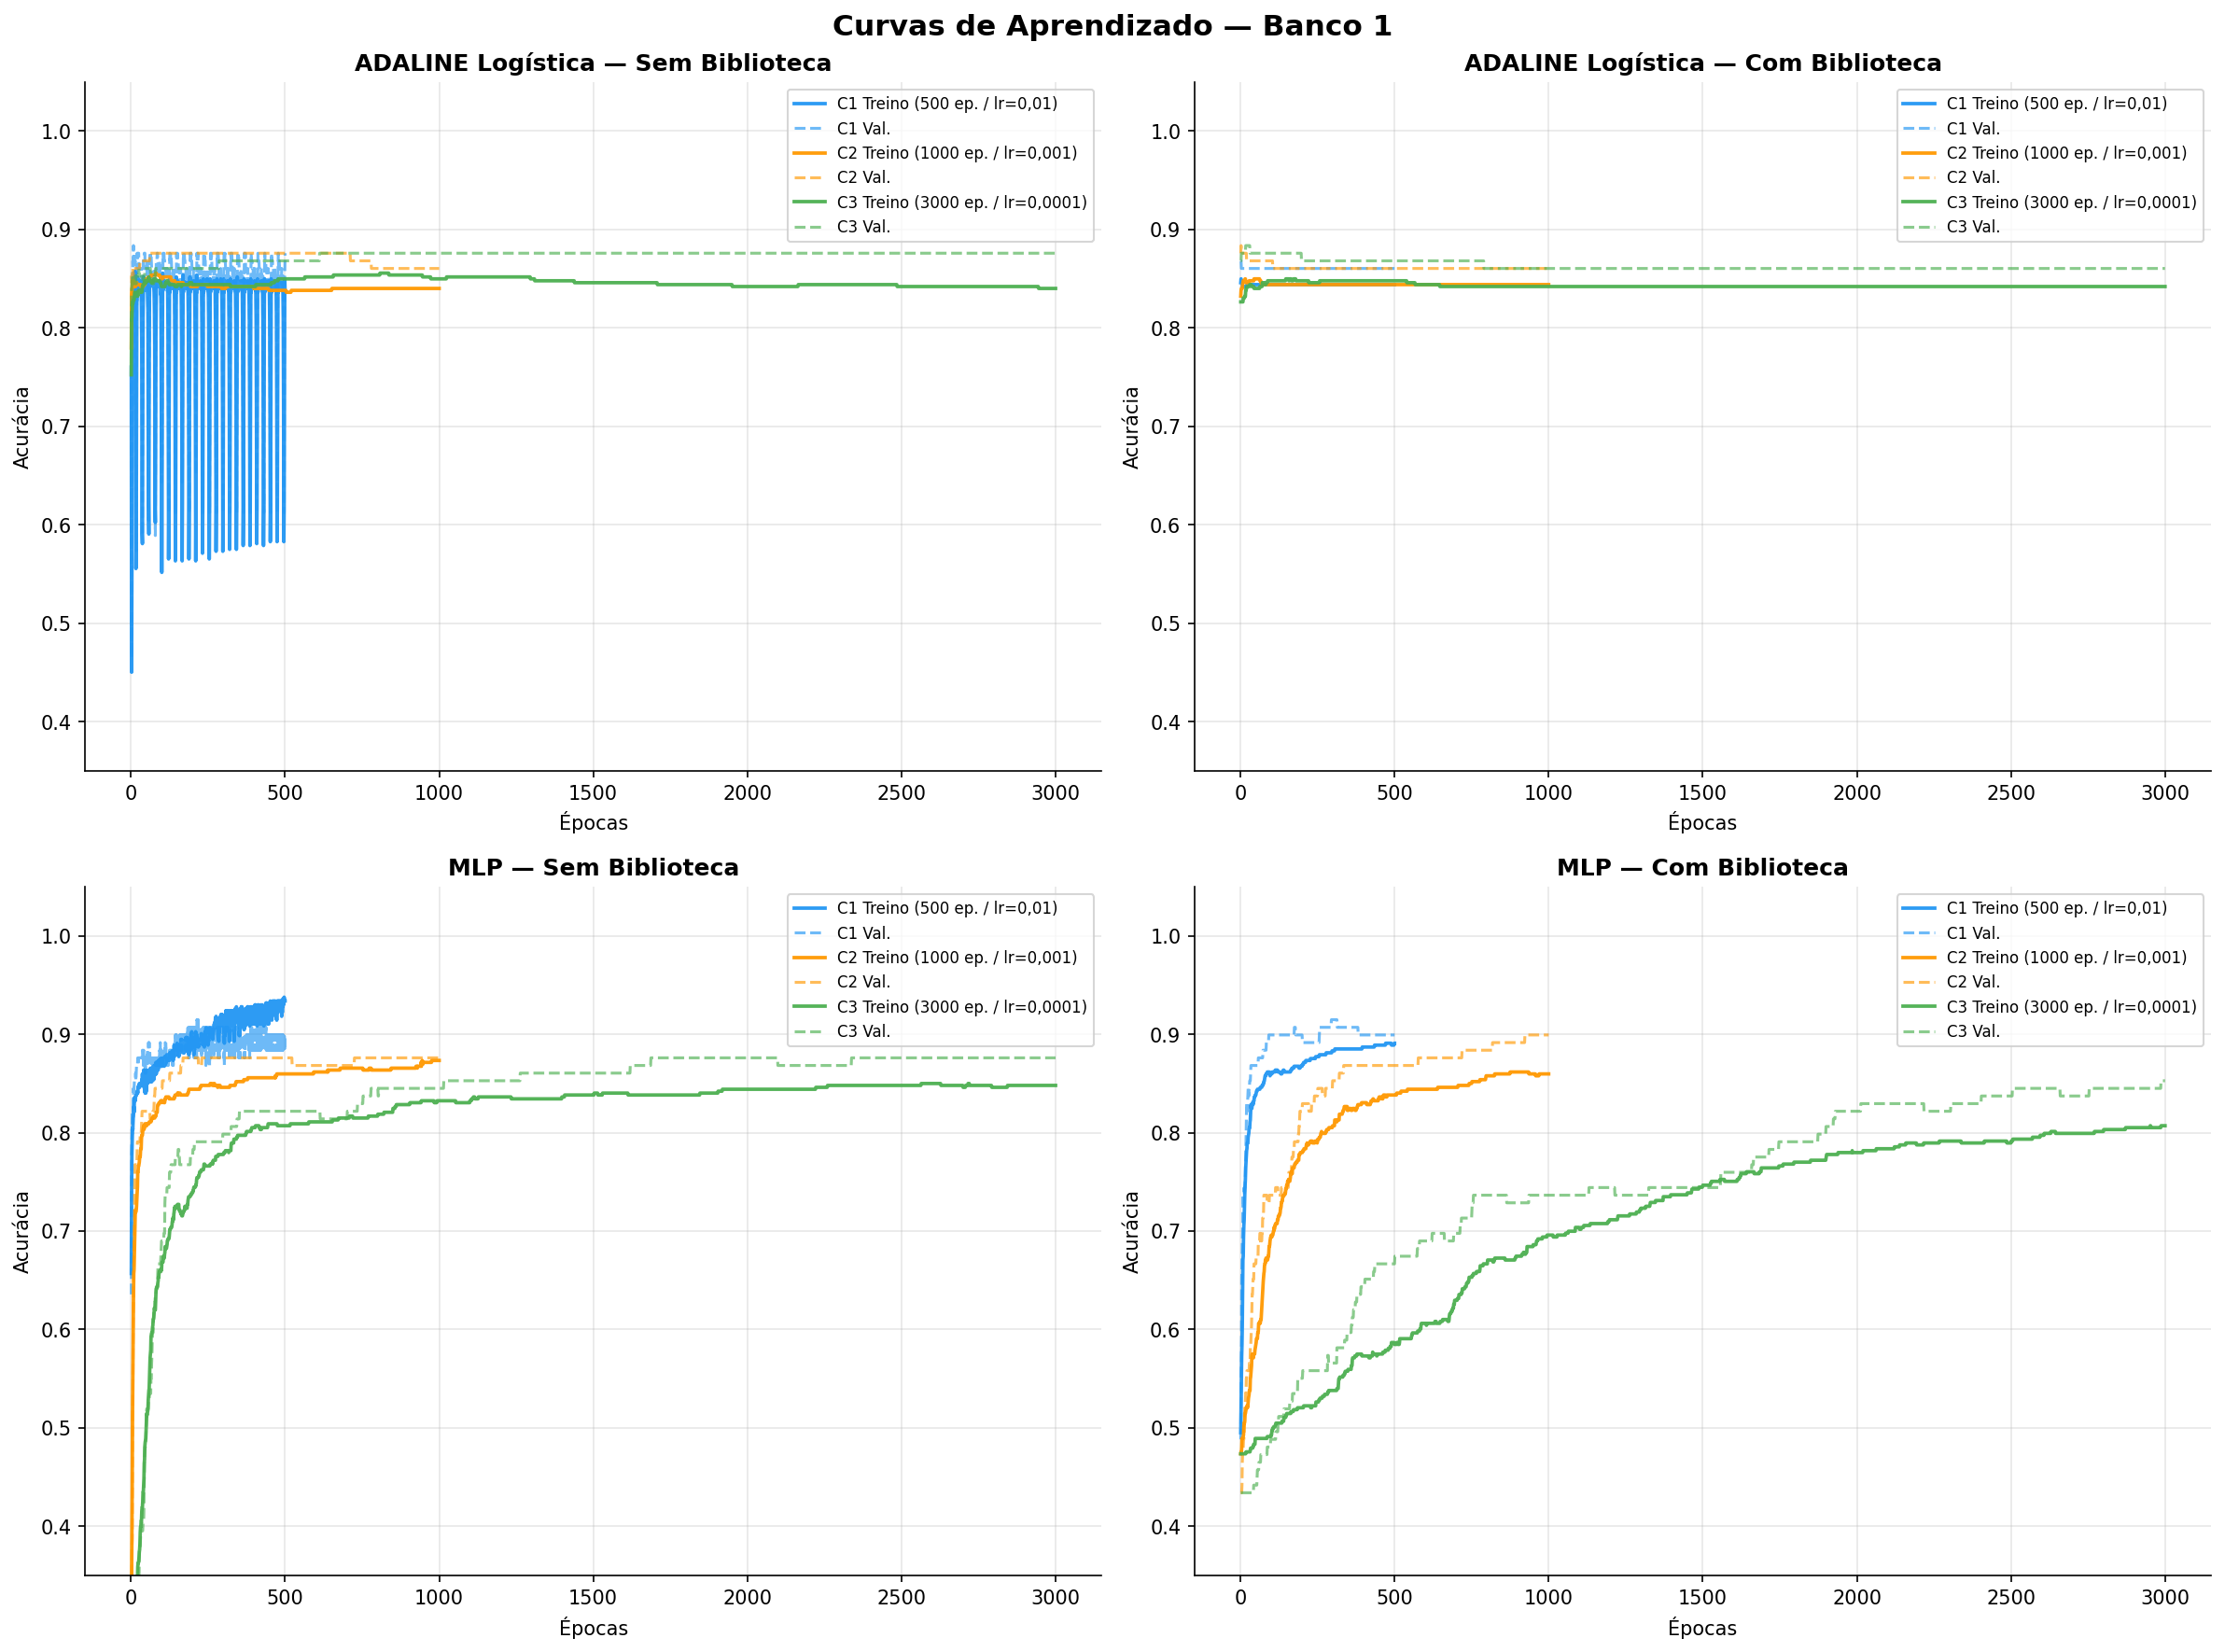
\includegraphics[width=\textwidth]{figuras/resultados/03_curvas_aprendizado_banco1.png}
\fonte{Elaborado pelo autor.}
\end{figure}

As curvas de aprendizado da Figura~\ref{fig:curvas_banco1} permitem observar o comportamento dinâmico de cada modelo ao longo das épocas. No painel do ADALINE NumPy, a configuração C1 exibe oscilações marcantes nas primeiras 500 épocas: a taxa de aprendizado elevada ($\eta = 0{,}01$) faz com que as atualizações de peso sejam grandes, provocando saltos na função de custo a cada época, comportamento característico do gradiente descendente em lote com taxa excessiva \cite{silva2016}. As configurações C2 e C3 convergem de forma suave, confirmando a estabilidade de taxas menores.

No painel do ADALINE Sklearn, as curvas são planas desde o início, com platô de validação atingido em menos de 200 épocas em todas as configurações, confirmando a convergência rápida do SGD.

O painel do MLP NumPy mostra progressão mais lenta mas consistente: a acurácia de treino e validação crescem juntas sem sinais de \textit{overfitting} (as curvas de treino e validação mantêm-se próximas), o que é esperado para gradiente descendente em lote que generaliza bem em conjuntos de tamanho moderado \cite{braga2007}. Já no painel do MLP Sklearn, observa-se para C3 um fenômeno típico de \textit{overfitting}: a curva de treino continua crescendo enquanto a curva de validação se estabiliza ou recua suavemente, indicando que o modelo começa a memorizar os exemplos de treino.

\subsection{Análise dos Falsos Negativos}
\label{sec:banco1_fn}

Conforme estabelecido na Seção~\ref{sec:metricas}, o Falso Negativo (FN), paciente doente classificado como saudável, representa o erro de maior impacto clínico neste contexto, pois implica a ausência de diagnóstico e tratamento em um paciente de risco. A Tabela~\ref{tab:fn_banco1} apresenta o total de FNs no conjunto de teste por modelo e configuração.

\begin{table}[H]
\centering
\caption[Falsos Negativos dos modelos no Banco 1 por configuração]{Total de Falsos Negativos (FN) dos modelos no Banco 1 por configuração de treinamento. Conjunto de teste: 276 pacientes (153 doentes / 123 saudáveis).}
\label{tab:fn_banco1}
\resizebox{\textwidth}{!}{%
\begin{tabular}{|l|c|c|c|}
\hline
\textbf{Modelo} & \textbf{C1 (500 ep., $\eta$=0,01)} & \textbf{C2 (1.000 ep., $\eta$=0,001)} & \textbf{C3 (3.000 ep., $\eta$=0,0001)} \\
\hline
ADALINE NumPy   & 28 & 21 & 20 \\
ADALINE Sklearn & 21 & 21 & 21 \\
MLP NumPy       & 27 & 16 & \textbf{15} \\
MLP Sklearn     & 18 & 20 & 35 \\
\hline
\end{tabular}}
\fonte{Elaborado pelo autor.}
\end{table}

A análise dos Falsos Negativos revela padrões distintos dos observados na acurácia, destacando a importância de não utilizar uma única métrica como critério de avaliação em aplicações clínicas \cite{braga2007}.

O ADALINE NumPy reduziu seus FNs progressivamente: 28 (C1) → 21 (C2) → 20 (C3). Esse comportamento é coerente com a melhora gradual da acurácia e com o fato de que a fronteira de decisão do ADALINE, ao ajustar os pesos, desloca-se em direção a uma região mais equilibrada entre sensibilidade e especificidade. Em 20 FNs, isso representa 13,07\% dos 153 pacientes doentes do conjunto de teste, um erro ainda clinicamente significativo, mas que reflete a limitação natural de um modelo linear em um problema com 35 características binárias.

O ADALINE Sklearn apresentou o comportamento mais rígido: 21 FNs em \textit{todas as configurações}, sem variação alguma. Esse resultado é notável: independentemente de se treinarem 500, 1.000 ou 3.000 épocas, e com taxas de aprendizado que variam 100 vezes (de 0,01 a 0,0001), o modelo sempre classificou incorretamente os mesmos 21 pacientes. Isso indica que o SGD atingiu um mínimo de custo específico que não é alterado por mudanças nos hiperparâmetros testados, o que pode ser interpretado como robustez do ponto de convergência, mas também como insensibilidade ao espaço de busca definido pelas configurações C1--C3.

O MLP NumPy obteve os melhores resultados clínicos do Banco 1: 27 FNs em C1, reduzindo para 16 em C2 e atingindo o mínimo de 15 FNs em C3. Esse progresso gradual é particularmente relevante porque a acurácia também melhorou no mesmo sentido (82,97\% → 87,68\%), o que significa que o modelo ganhou em ambas as dimensões simultaneamente. Com 15 FNs em 153 doentes, a sensibilidade alcança 90,20\%, significando que 9 em cada 10 pacientes doentes são corretamente identificados como doentes na configuração C3.

O MLP Sklearn demonstrou o comportamento mais problemático clinicamente: embora tenha iniciado com bons resultados em C1 (18 FNs), degradou-se progressivamente para 20 em C2 e chegou ao pior resultado do Banco 1 com 35 FNs em C3. Esse número representa 22,88\% dos pacientes doentes sendo classificados como saudáveis, quase um em cada quatro doentes não detectados. Esse resultado contradiz diretamente a acurácia de C1 (87,32\%) e demonstra que a otimização de acurácia global não garante minimização de FNs.

A Figura~\ref{fig:matrizes_banco1} apresenta as matrizes de confusão de todos os modelos na configuração C3 (3.000 épocas, $\eta = 0{,}0001$). Essa configuração foi adotada como referência de visualização por ser aquela em que as diferenças de comportamento clínico entre os modelos se manifestam de forma mais acentuada: em particular, a degradação do MLP Sklearn, com 35 Falsos Negativos em C3 contra 18 em C1, torna-se visível nas matrizes e faz da comparação entre arquiteturas nessa configuração a mais informativa dentre as três estudadas.

\begin{figure}[H]
\centering
\caption[Matrizes de confusão dos modelos, Banco 1, configuração C3.]{Matrizes de confusão dos quatro modelos no Banco 1, configuração C3 (3.000 épocas, $\eta$ = 0,0001).}
\label{fig:matrizes_banco1}
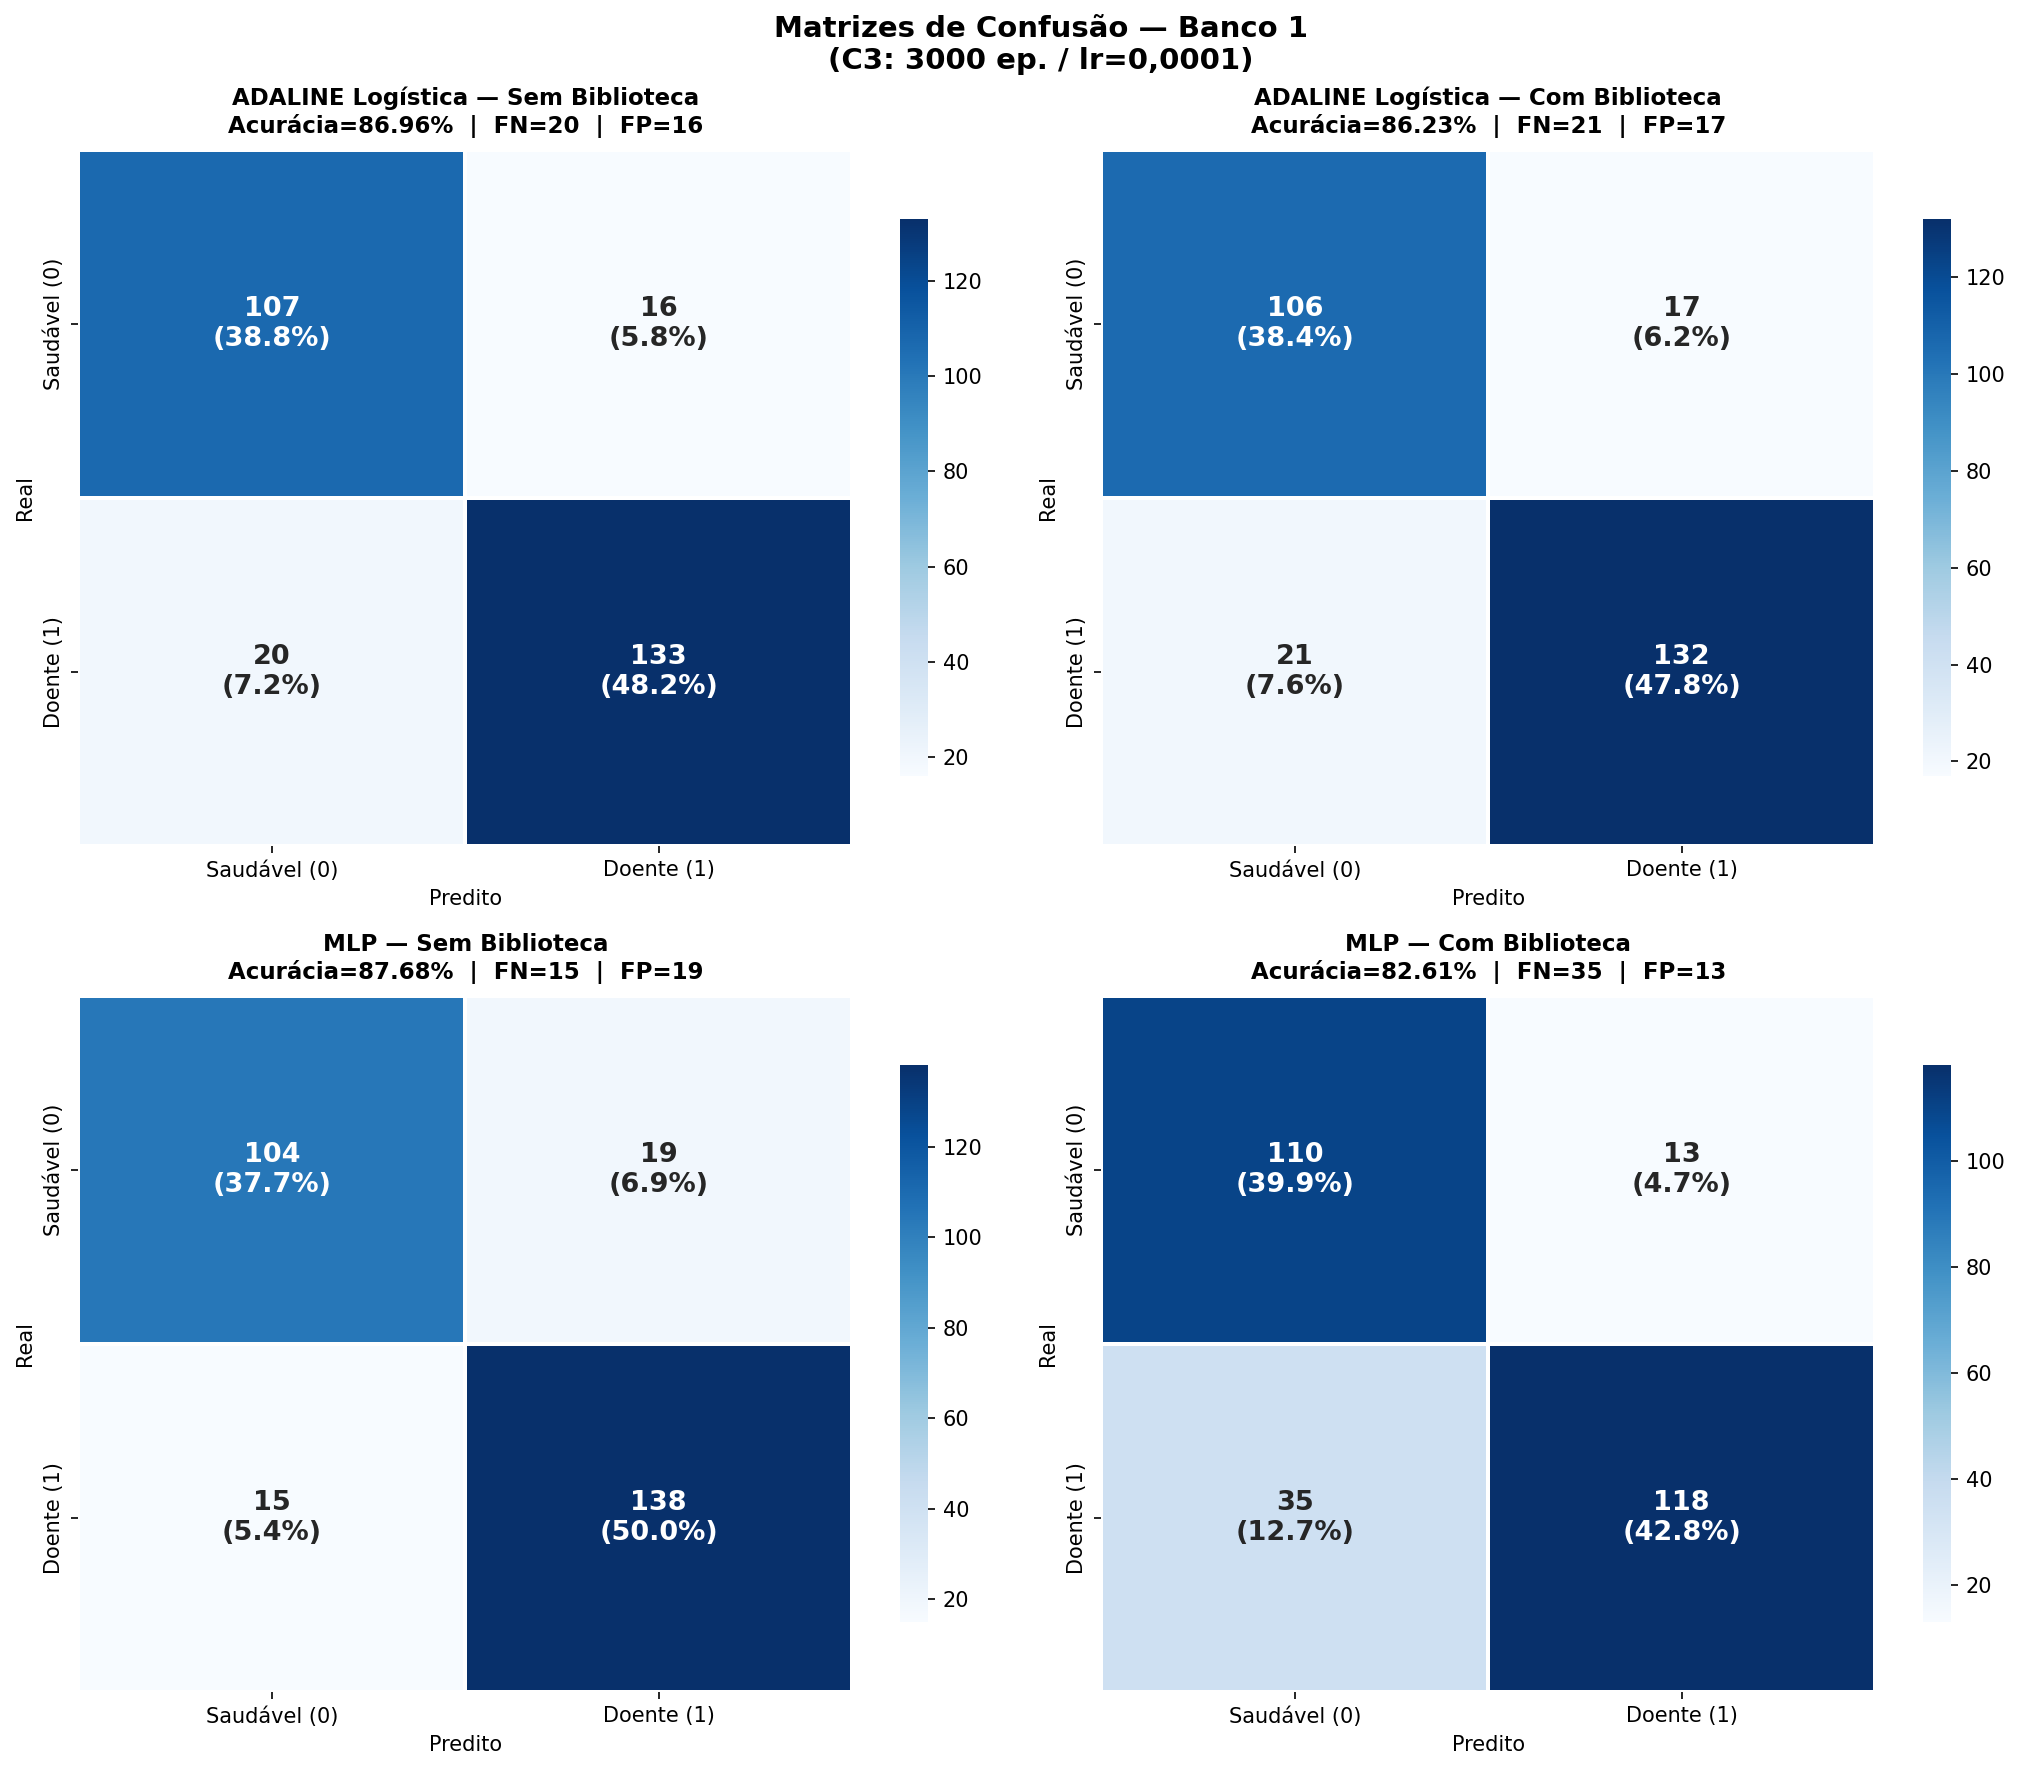
\includegraphics[width=\textwidth]{figuras/resultados/07_matrizes_confusao_banco1.png}
\fonte{Elaborado pelo autor.}
\end{figure}

A partir das matrizes de confusão da Figura~\ref{fig:matrizes_banco1} e dos valores de VP, VN, FP e FN, é possível calcular as métricas complementares de sensibilidade, especificidade e precisão. A Tabela~\ref{tab:metricas_banco1_c3} consolida esses valores para C3.

\begin{table}[H]
\centering
\caption{Métricas de avaliação dos modelos no Banco 1, configuração C3. Conjunto de teste: 276 pacientes.}
\label{tab:metricas_banco1_c3}
\begin{tabular}{|l|c|c|c|c|c|c|c|}
\hline
\textbf{Modelo} & \textbf{VP} & \textbf{VN} & \textbf{FP} & \textbf{FN} & \textbf{Sensib.} & \textbf{Especif.} & \textbf{Precisão} \\
\hline
ADALINE NumPy   & 133 & 107 & 16 & 20 & 86,93\% & 86,99\% & 89,26\% \\
ADALINE Sklearn & 132 & 106 & 17 & 21 & 86,27\% & 86,18\% & 88,59\% \\
MLP NumPy       & 138 & 104 & 19 & 15 & \textbf{90,20\%} & 84,55\% & 87,90\% \\
MLP Sklearn     & 118 & 110 & 13 & 35 & 77,12\% & \textbf{89,43\%} & 90,08\% \\
\hline
\end{tabular}
\fonte{Elaborado pelo autor.}
\vspace*{-\baselineskip}
\end{table}

A Tabela~\ref{tab:metricas_banco1_c3} evidencia um contraste fundamental entre os modelos em C3. O MLP NumPy atingiu a maior sensibilidade (90,20\%), identificando corretamente 138 dos 153 pacientes doentes, resultado clinicamente mais relevante. O MLP Sklearn, por sua vez, apresentou a maior especificidade (89,43\%) e precisão (90,08\%), mas ao custo de uma sensibilidade muito inferior (77,12\%) e do maior número de FNs (35). Isso revela que o MLP Sklearn em C3 aprendeu a ser conservador na predição de doença, classificando mais pacientes como saudáveis, o que reduz os FPs e aumenta a especificidade, mas eleva os FNs a níveis clinicamente inaceitáveis. Os dois modelos ADALINE apresentaram sensibilidade e especificidade equilibradas (ambas próximas de 87\%), comportamento coerente com a natureza simétrica da função logística e com a convergência estável da regra delta.

\subsection{Convergência do Erro de Treinamento}
\label{sec:banco1_convergencia}

A Figura~\ref{fig:convergencia_banco1} apresenta a evolução do Erro Quadrático Médio (MSE) ao longo das épocas de treinamento para os quatro modelos no Banco 1, permitindo comparar a velocidade de convergência e a estabilidade de cada abordagem.

\begin{figure}[H]
\centering
\caption{Convergência do Erro Quadrático Médio (MSE) por época nos quatro modelos, Banco 1.}
\label{fig:convergencia_banco1}
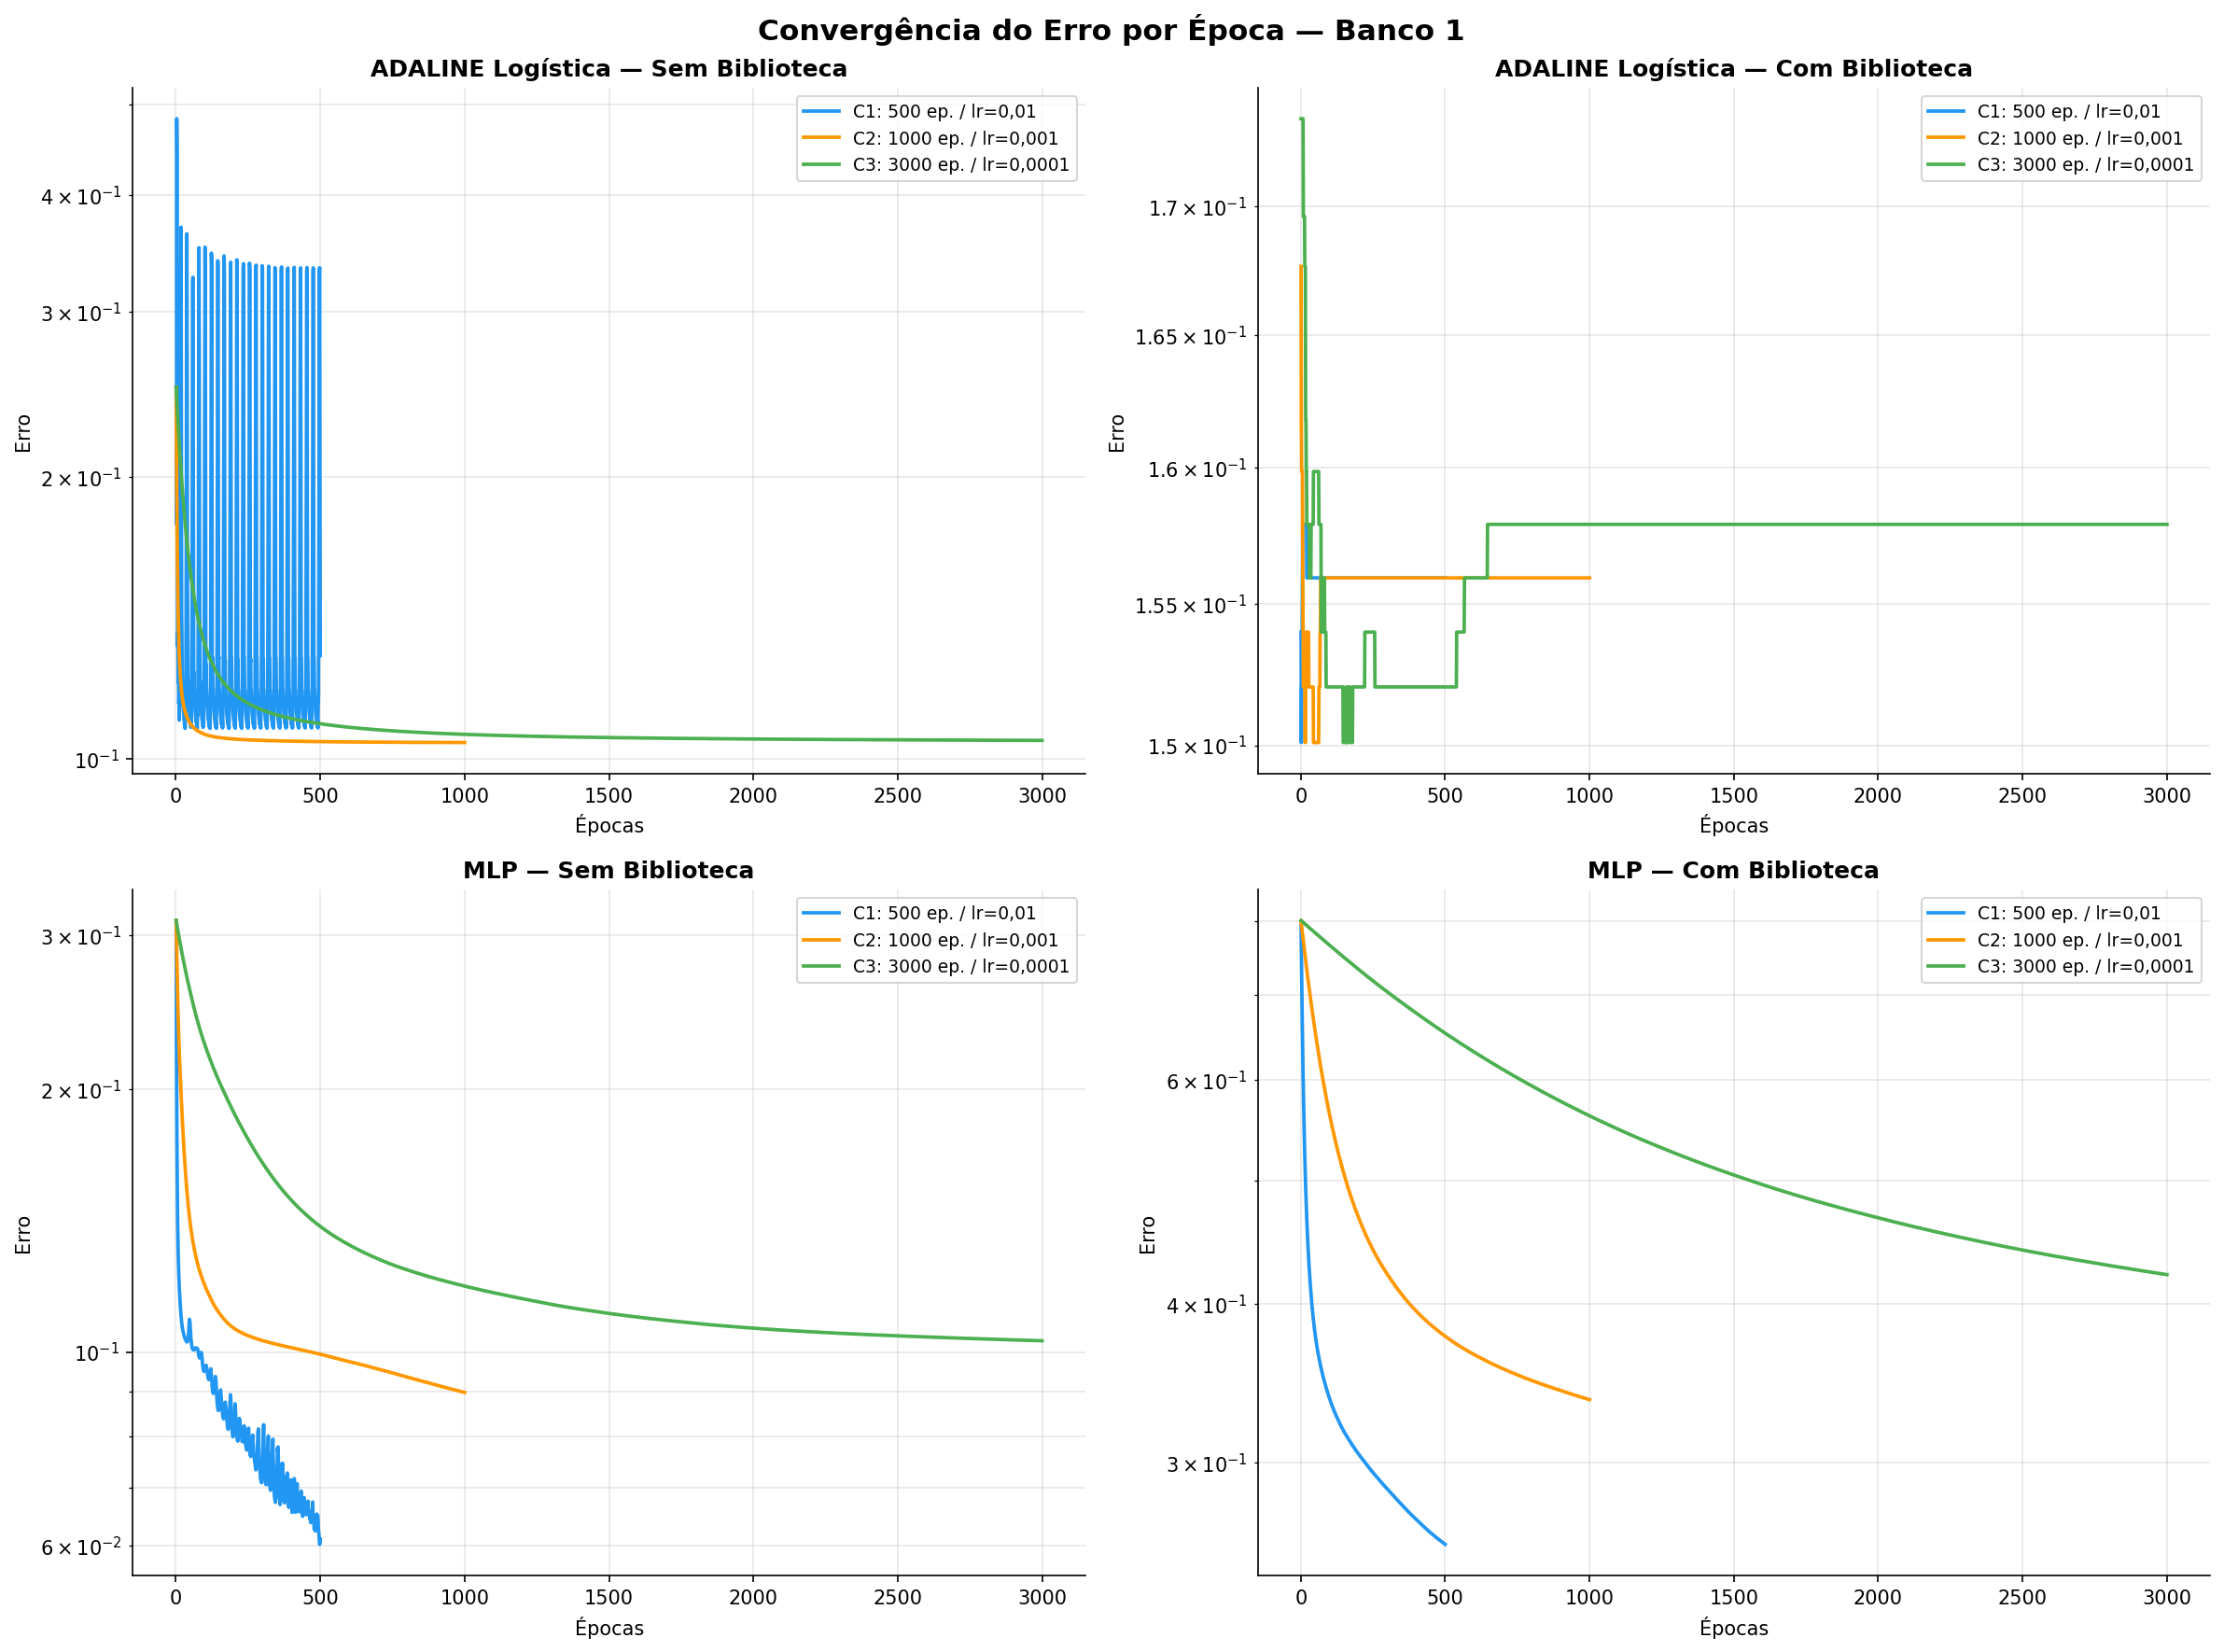
\includegraphics[width=\textwidth]{figuras/resultados/05_convergencia_erro_banco1.png}
\fonte{Elaborado pelo autor.}
\end{figure}

A Figura~\ref{fig:convergencia_banco1} ilustra a evolução do MSE de treinamento ao longo das épocas. Dois comportamentos contrastantes são imediatamente visíveis.

No painel do ADALINE NumPy, a configuração C1 ($\eta = 0{,}01$) exibe oscilações de grande amplitude nas primeiras épocas, com o erro chegando a valores próximos de $4 \times 10^{-1}$ antes de decair. Essas oscilações decorrem diretamente da taxa de aprendizado elevada em combinação com o gradiente calculado sobre todo o conjunto de treinamento (modo lote): quando $\eta$ é grande, cada passo de gradiente pode ultrapassar o mínimo da função de custo, fazendo o erro oscilar antes de convergir. As configurações C2 e C3 convergem suavemente e de forma monotônica, confirmando que taxas menores produzem trajetórias mais estáveis, ainda que mais lentas \cite{silva2016}.

No painel do ADALINE Sklearn, as três curvas são planas e estacionárias desde o início, coerentes com o comportamento de acurácia observado na Seção~\ref{sec:banco1_acuracia}.

Os painéis do MLP NumPy e MLP Sklearn mostram curvas de convergência mais lentas e com patamares distintos. Para o MLP NumPy, as três configurações apresentam convergência suave e monotônica, com C1 atingindo erro maior (ainda convergindo mais lentamente por ter apenas 500 épocas), C2 chegando a um nível intermediário e C3 atingindo o menor erro final, consistente com os melhores resultados de acurácia e FNs em C3. Para o MLP Sklearn, a curva de C3 apresenta erro decrescente ao longo das 3.000 épocas sem sinais de estabilização, o que, combinado com a acurácia de validação estacionária (Figura~\ref{fig:curvas_banco1}), é sinal inequívoco de \textit{overfitting}: o modelo está reduzindo o erro de treino enquanto a capacidade de generalização piora \cite{dsa2022}.

\section{Banco 2 --- Heart Failure Clinical Records}
\label{sec:resultados_banco2}

O Banco 2 contém 299 registros de pacientes com insuficiência cardíaca diagnosticada, com objetivo de prognóstico de mortalidade (\textit{DEATH\_EVENT}). Após a divisão estratificada, o conjunto de teste compreende 90 pacientes: 61 sobreviventes (67,8\%) e 29 óbitos (32,2\%). O volume significativamente menor (299 versus 918 do Banco 1), o desequilíbrio de classes mais acentuado (33\% versus 45\% de positivos) e a natureza mais complexa do objetivo preditivo, prognóstico de óbito em vez de triagem diagnóstica, tornam este banco intrinsecamente mais desafiador \cite{chicco2020}.

\subsection{Acurácia por Configuração de Treinamento}
\label{sec:banco2_acuracia}

A Tabela~\ref{tab:acuracia_banco2} apresenta a acurácia percentual de cada modelo nas três configurações de treinamento para o Banco 2. O padrão de desempenho difere fundamentalmente do Banco 1: as acurácias globais são menores e as trajetórias dos modelos MLP ao longo das configurações são inversas ao comportamento observado anteriormente, com degradação progressiva do desempenho à medida que o treinamento se estende.

\begin{table}[H]
\centering
\caption{Acurácia (\%) dos modelos no Banco 2 por configuração de treinamento.}
\label{tab:acuracia_banco2}
\resizebox{\textwidth}{!}{%
\begin{tabular}{|l|c|c|c|}
\hline
\textbf{Modelo} & \textbf{C1 (500 ep., $\eta$=0,01)} & \textbf{C2 (1.000 ep., $\eta$=0,001)} & \textbf{C3 (3.000 ep., $\eta$=0,0001)} \\
\hline
ADALINE NumPy   & 68,89\% & 72,22\% & \textbf{75,56\%} \\
ADALINE Sklearn & 68,89\% & 68,89\% & 68,89\% \\
MLP NumPy       & \textbf{78,89\%} & 75,56\% & 71,11\% \\
MLP Sklearn     & 73,33\% & 68,89\% & 63,33\% \\
\hline
\end{tabular}}
\fonte{Elaborado pelo autor.}
\end{table}

O ADALINE NumPy é o único modelo cujo desempenho melhora monotonicamente: 68,89\% → 72,22\% → 75,56\%. Esse comportamento reflete a estabilidade do gradiente descendente em lote com taxas conservadoras em conjuntos pequenos, o modelo ajusta a fronteira linear lentamente mas sem instabilidade \cite{silva2016}.

O ADALINE Sklearn repetiu o comportamento de rigidez observado no Banco 1, mas de forma ainda mais extrema: acurácia idêntica de 68,89\% em \textit{todas as três configurações}, sem qualquer variação. Em um conjunto de 90 pacientes de teste, isso equivale a exatamente 62 classificações corretas em todas as situações. O SGD converge para um mínimo específico nas primeiras épocas e permanece estacionário, insensível a qualquer ajuste de hiperparâmetros dentro do espaço testado. Esse comportamento, que no Banco 1 poderia ser interpretado como convergência robusta, no Banco 2 é mais indicativo de uma limitação: o modelo está preso em uma solução subótima que não consegue sair \cite{pedregosa2011}.

O MLP NumPy apresentou o resultado inverso ao esperado: a melhor configuração foi C1 (78,89\%), e o desempenho degradou progressivamente em C2 (75,56\%) e C3 (71,11\%). Esse fenômeno é um caso claro de \textit{overfitting} induzido por treinamento excessivo em um conjunto de dados pequeno: com apenas 167 exemplos efetivos de treinamento (correspondentes a 80\% dos 209 pacientes do conjunto de treino obtido pela divisão 70/30), 3.000 épocas representam 3.000 passagens completas pelo conjunto de treino de 167 exemplos, número excessivo para um conjunto tão pequeno com gradiente descendente em lote. O modelo passa a memorizar os exemplos individuais de treino em vez de aprender padrões generalizáveis \cite{braga2007}.

O MLP Sklearn apresentou a degradação mais severa de todos: 73,33\% em C1, caindo para 68,89\% em C2 e chegando ao mínimo de 63,33\% em C3, a menor acurácia de todos os experimentos. O SGD com momento ($\beta = 0{,}9$), com sua velocidade acumulada que continua impulsionando os parâmetros mesmo em fases avançadas do treinamento, é particularmente suscetível a \textit{overfitting} em datasets pequenos: sem dados suficientes para regularizar o aprendizado, a velocidade acumulada ajusta os pesos excessivamente aos exemplos de treino \cite{dsa2022}.

\begin{figure}[H]
\centering
\caption{Curvas de aprendizado (acurácia de treino e validação) dos quatro modelos no Banco 2 para as três configurações de treinamento.}
\label{fig:curvas_banco2}
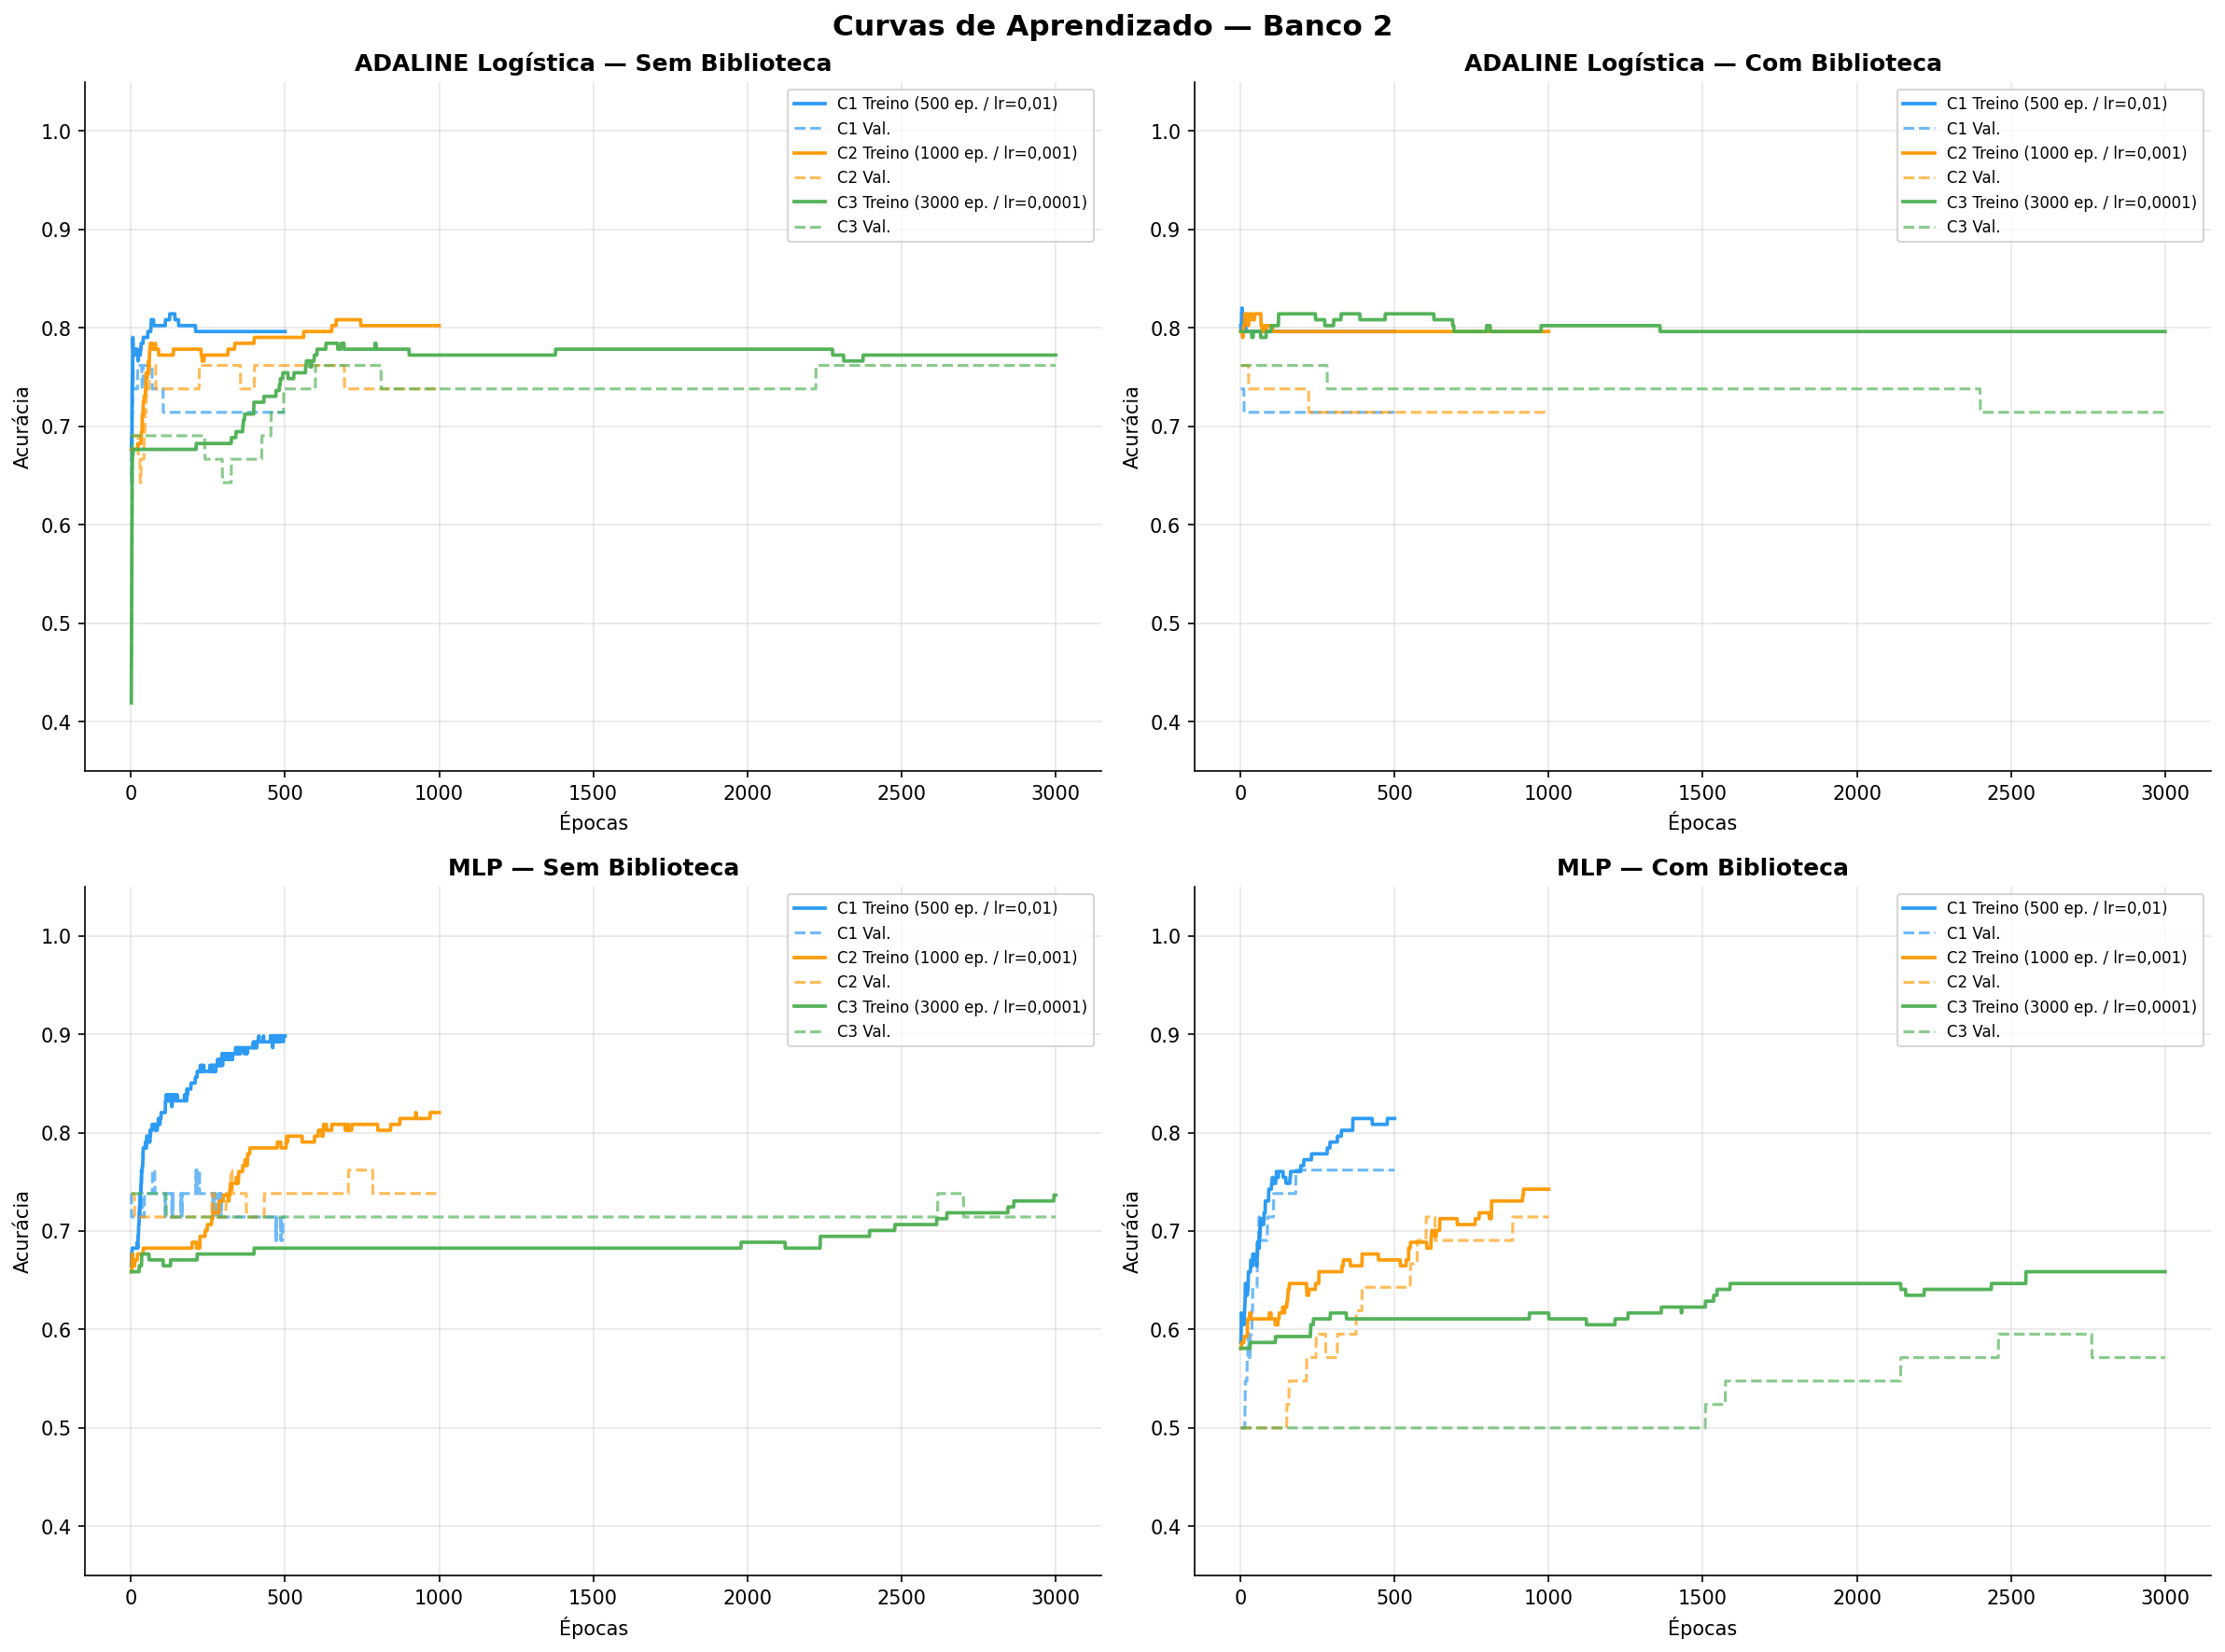
\includegraphics[width=\textwidth]{figuras/resultados/04_curvas_aprendizado_banco2.png}
\fonte{Elaborado pelo autor.}
\end{figure}

A Figura~\ref{fig:curvas_banco2} evidencia o \textit{overfitting} dos modelos MLP: em C3, a acurácia de treino continua crescendo enquanto a de validação oscila ou recua, com divergência especialmente pronunciada no MLP Sklearn. O comportamento escalonado do ADALINE Sklearn confirma a rigidez do SGD.

\subsection{Análise dos Falsos Negativos}
\label{sec:banco2_fn}

Neste banco, em que a classe positiva corresponde aos óbitos, apenas 29 dos 90 pacientes do conjunto de teste, a análise dos Falsos Negativos assume especial relevância clínica. Cada FN representa um paciente que veio a óbito mas foi classificado como sobrevivente pelo modelo, erro que poderia implicar a ausência de intervenção terapêutica em tempo oportuno. A Tabela~\ref{tab:fn_banco2} apresenta o total de FNs por modelo e configuração.

\begin{table}[H]
\centering
\caption[Falsos Negativos dos modelos no Banco 2 por configuração]{Total de Falsos Negativos (FN) dos modelos no Banco 2 por configuração de treinamento. Conjunto de teste: 90 pacientes (29 óbitos / 61 sobreviventes).}
\label{tab:fn_banco2}
\resizebox{\textwidth}{!}{%
\begin{tabular}{|l|c|c|c|}
\hline
\textbf{Modelo} & \textbf{C1 (500 ep., $\eta$=0,01)} & \textbf{C2 (1.000 ep., $\eta$=0,001)} & \textbf{C3 (3.000 ep., $\eta$=0,0001)} \\
\hline
ADALINE NumPy   & 17 & 17 & 16 \\
ADALINE Sklearn & 17 & 17 & 17 \\
MLP NumPy       & \textbf{9}  & 14 & 23 \\
MLP Sklearn     & 18 & 17 & \textbf{8} \\
\hline
\end{tabular}}
\fonte{Elaborado pelo autor.}
\end{table}

A Tabela~\ref{tab:fn_banco2} revela um dos resultados mais intrigantes de todo o trabalho: o MLP Sklearn em C3, que apresentou a \textit{pior} acurácia (63,33\%), produziu simultaneamente o \textit{menor} número de Falsos Negativos (8 FNs). Aparentemente contraditório, esse resultado é explicado pela análise das matrizes de confusão (Figura~\ref{fig:matrizes_banco2}): o modelo aprendeu a classificar uma proporção elevada de pacientes como doentes (\textit{DEATH\_EVENT} = 1), o que reduz os FNs ao custo de inflar dramaticamente os Falsos Positivos. Trata-se de uma troca desfavorável para uso clínico, pois pacientes saudáveis são alarmados desnecessariamente, mas que ilustra como a escolha da métrica de avaliação principal influencia a interpretação do desempenho de um modelo \cite{braga2007}.

O MLP NumPy em C1 obteve o melhor equilíbrio entre acurácia e FNs no Banco 2: 78,89\% de acurácia e apenas 9 FNs, representando 31,03\% de falhas na detecção de óbitos. Isso equivale a uma sensibilidade de 68,97\%, o melhor resultado geral deste banco de dados. A degradação progressiva do MLP NumPy em C2 (14 FNs) e C3 (23 FNs) confirma o \textit{overfitting}: à medida que o modelo se especializa nos exemplos de treino, começa a errar em exemplos de teste que não foram memorizados, e por ser a classe de óbito a minoria (33\%), os erros tendem a recair desproporcionalmente sobre ela.

Os modelos ADALINE mantiveram FNs estáveis em torno de 16--17 em todas as configurações, coerente com a fronteira de decisão linear que não se altera significativamente entre as configurações. Com 17 FNs em 29 óbitos, a sensibilidade do ADALINE Sklearn é de 41,38\%, diagnosticando corretamente apenas 2 em cada 5 pacientes que vieram a óbito. Embora este número seja clinicamente preocupante, ele reflete a dificuldade inerente do problema: prever óbito em pacientes com insuficiência cardíaca a partir de dados clínicos tabulares e binários é uma tarefa com alto grau de incerteza, e a acurácia de 75,56\% atingida pelo ADALINE NumPy em C3, com apenas 16 FNs, representa o melhor compromisso entre confiabilidade global e detecção de casos críticos neste banco \cite{chicco2020}.

Dado que a configuração C1 representa o melhor desempenho geral do Banco 2, a Tabela~\ref{tab:metricas_banco2_c1} detalha as métricas consolidadas para essa configuração, derivadas das contagens de VP, VN, FP e FN calculadas a partir da acurácia e dos FNs apresentados nas Tabelas~\ref{tab:acuracia_banco2} e \ref{tab:fn_banco2}.

\begin{table}[H]
\centering
\caption{Métricas de avaliação dos modelos no Banco 2, configuração C1. Conjunto de teste: 90 pacientes (29 óbitos / 61 sobreviventes).}
\label{tab:metricas_banco2_c1}
\begin{tabular}{|l|c|c|c|c|c|c|c|}
\hline
\textbf{Modelo} & \textbf{VP} & \textbf{VN} & \textbf{FP} & \textbf{FN} & \textbf{Sensib.} & \textbf{Especif.} & \textbf{Precisão} \\
\hline
ADALINE NumPy   & 12 & 50 & 11 & 17 & 41,38\% & 81,97\% & 52,17\% \\
ADALINE Sklearn & 12 & 50 & 11 & 17 & 41,38\% & 81,97\% & 52,17\% \\
MLP NumPy       & 20 & 51 & 10 &  9 & \textbf{68,97\%} & 83,61\% & 66,67\% \\
MLP Sklearn     & 11 & 55 &  6 & 18 & 37,93\% & \textbf{90,16\%} & 64,71\% \\
\hline
\end{tabular}
\fonte{Elaborado pelo autor.}
\end{table}

A Tabela~\ref{tab:metricas_banco2_c1} confirma que o MLP NumPy em C1 oferece o melhor equilíbrio entre sensibilidade (68,97\%) e especificidade (83,61\%), identificando 20 dos 29 óbitos com apenas 10 falsos alarmes. O MLP Sklearn em C1, apesar de boa especificidade (90,16\%), apresenta a pior sensibilidade (37,93\%), menos de 4 em cada 10 óbitos detectados. Os dois modelos ADALINE são idênticos em C1, com sensibilidade de 41,38\% e especificidade de 81,97\%, resultado da mesma convergência atingida pelo gradiente descendente e pelo SGD nessa configuração.

\begin{figure}[H]
\centering
\caption[Matrizes de confusão dos modelos, Banco 2, configuração C3.]{Matrizes de confusão dos quatro modelos no Banco 2, configuração C3 (3.000 épocas, $\eta$ = 0,0001).}
\label{fig:matrizes_banco2}
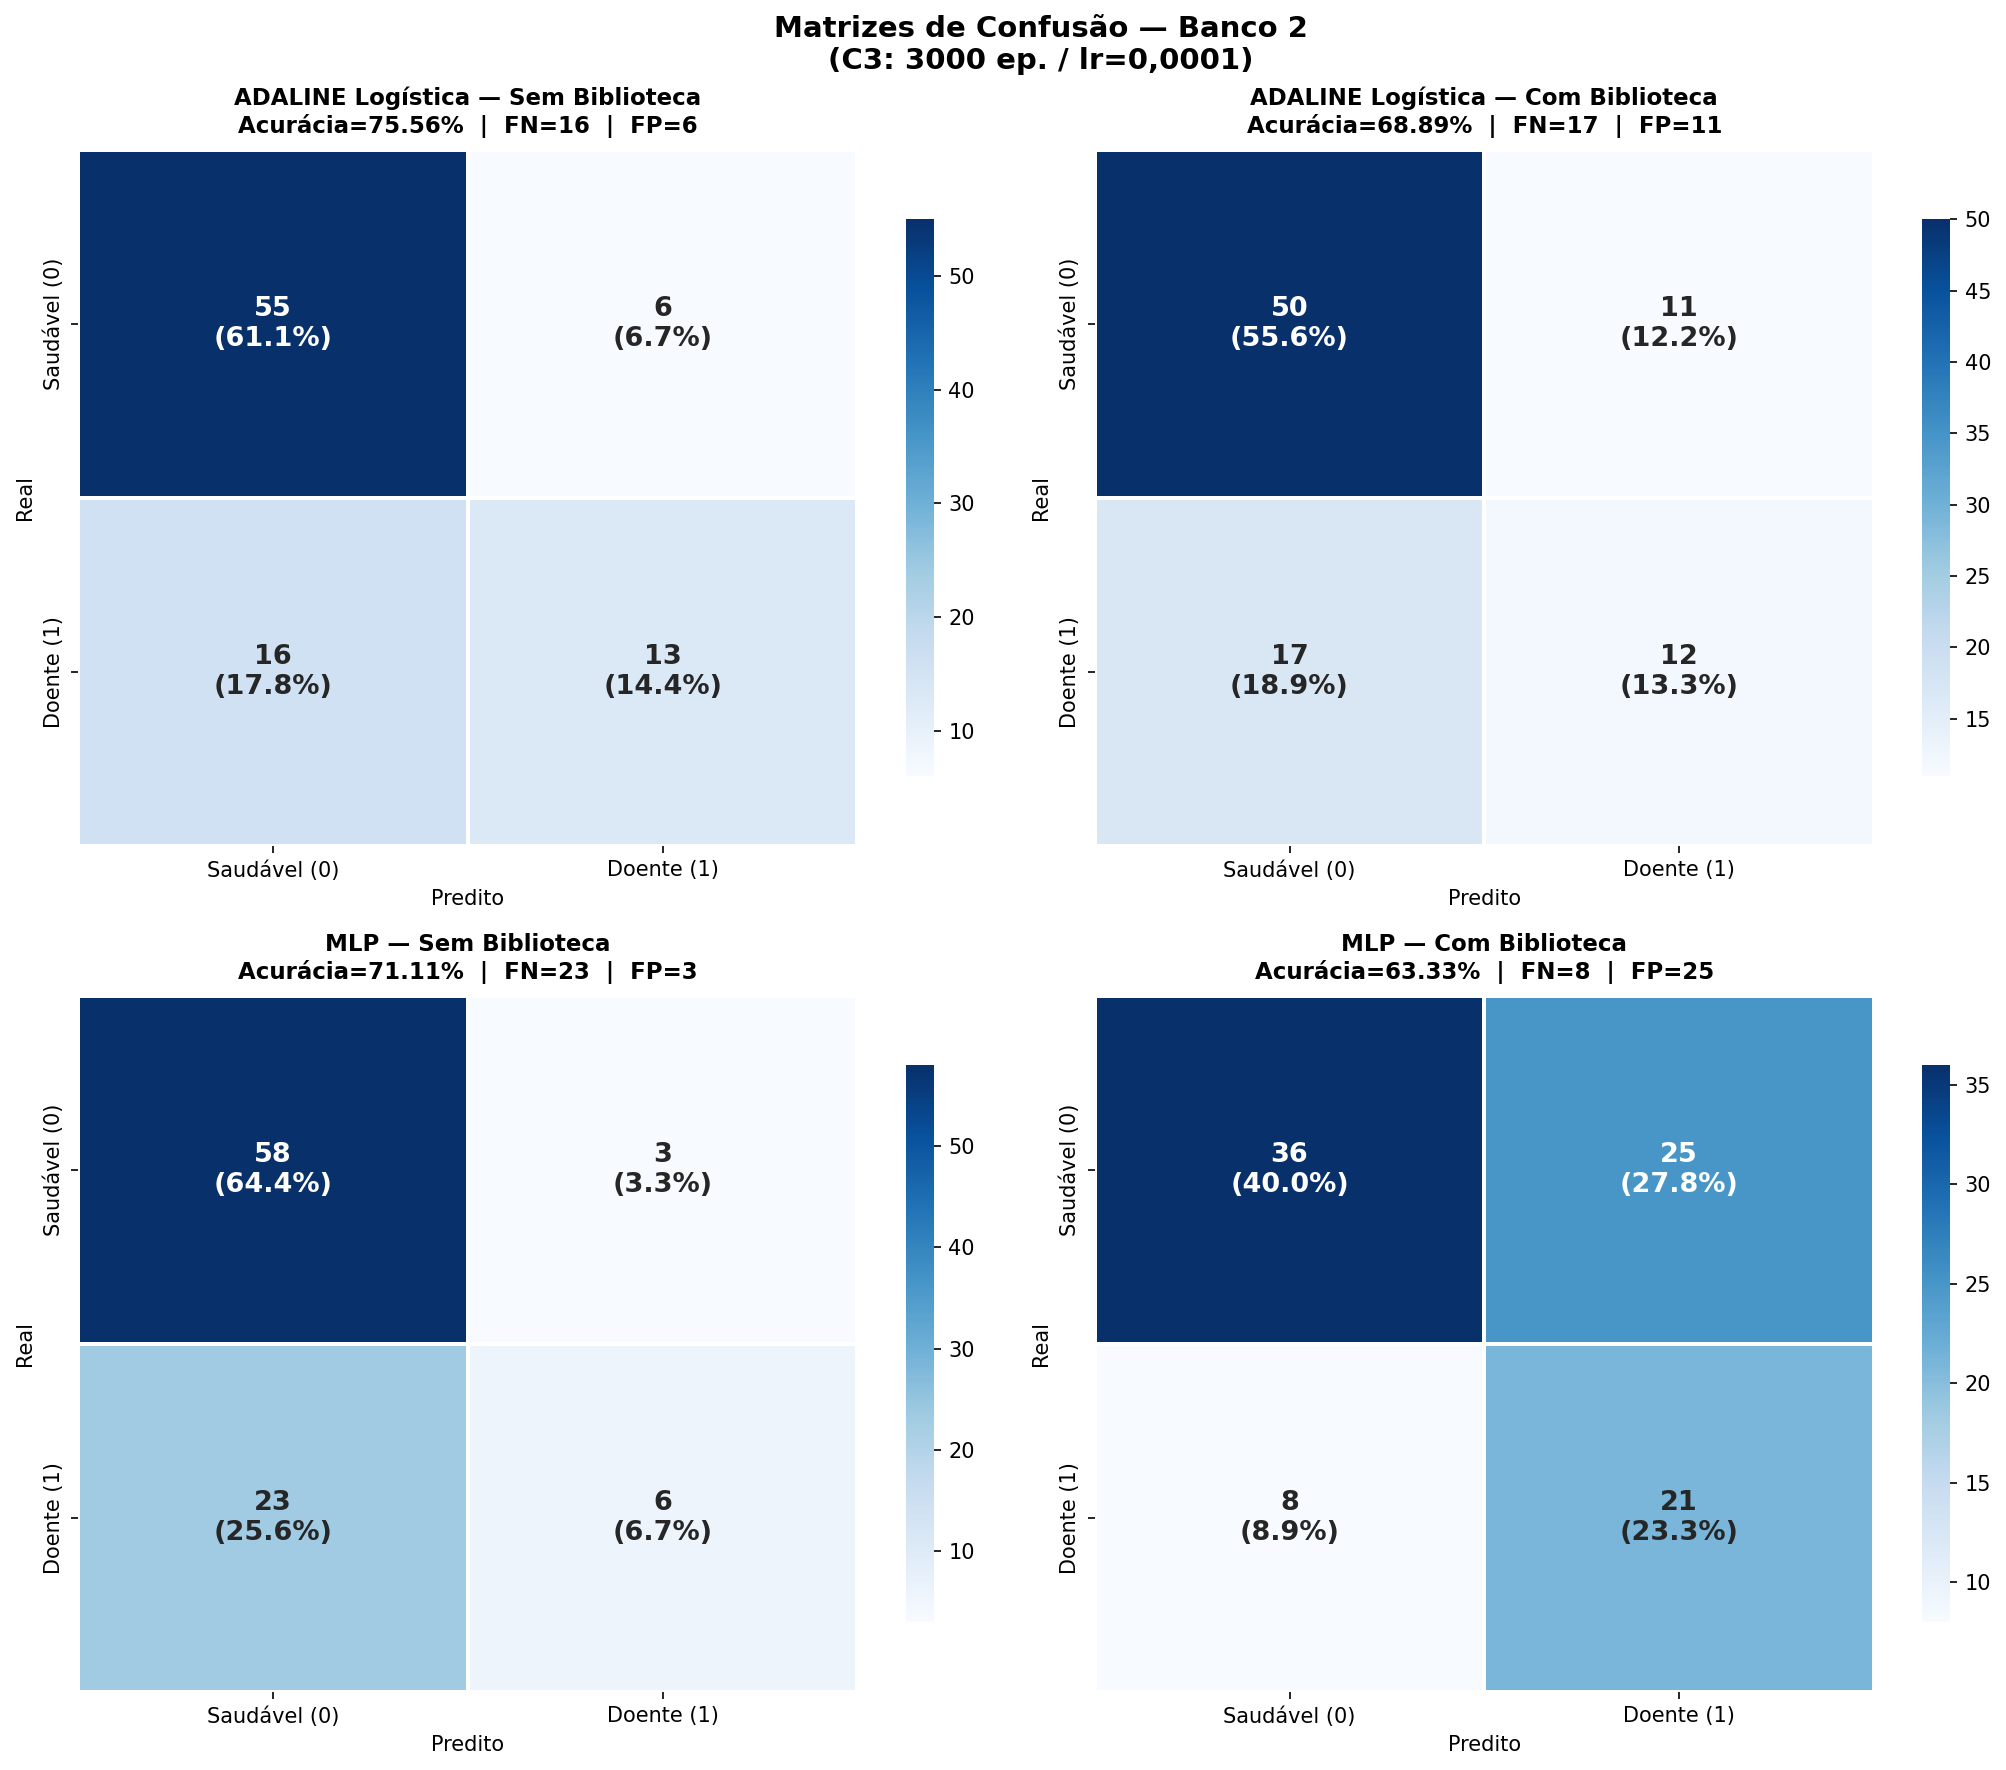
\includegraphics[width=\textwidth]{figuras/resultados/08_matrizes_confusao_banco2.png}
\fonte{Elaborado pelo autor.}
\end{figure}

A Tabela~\ref{tab:metricas_banco2_c3} consolida as métricas de avaliação para C3 calculadas a partir das matrizes de confusão da Figura~\ref{fig:matrizes_banco2}.

\begin{table}[H]
\centering
\caption{Métricas de avaliação dos modelos no Banco 2, configuração C3. Conjunto de teste: 90 pacientes.}
\label{tab:metricas_banco2_c3}
\begin{tabular}{|l|c|c|c|c|c|c|c|}
\hline
\textbf{Modelo} & \textbf{VP} & \textbf{VN} & \textbf{FP} & \textbf{FN} & \textbf{Sensib.} & \textbf{Especif.} & \textbf{Precisão} \\
\hline
ADALINE NumPy   & 13 & 55 & 6  & 16 & 44,83\% & \textbf{90,16\%} & 68,42\% \\
ADALINE Sklearn & 12 & 50 & 11 & 17 & 41,38\% & 81,97\% & 52,17\% \\
MLP NumPy       & 6  & 58 & 3  & 23 & 20,69\% & 95,08\% & 66,67\% \\
MLP Sklearn     & 21 & 36 & 25 & \textbf{8}  & \textbf{72,41\%} & 59,02\% & 45,65\% \\
\hline
\end{tabular}
\fonte{Elaborado pelo autor.}
\end{table}

Os dados da Tabela~\ref{tab:metricas_banco2_c3} expõem a tensão entre sensibilidade e especificidade no Banco 2. O MLP Sklearn em C3 atinge a maior sensibilidade (72,41\%), mas com especificidade de apenas 59,02\%, ou seja, 4 em cada 10 pacientes saudáveis são incorretamente classificados como doentes. O MLP NumPy em C3, por outro lado, atinge especificidade de 95,08\% (quase nenhum falso alarme), mas sensibilidade de apenas 20,69\%, identificando apenas 1 em cada 5 pacientes que vieram a óbito. Esse contraste confirma que, para o Banco 2 em C3, nenhum modelo atingiu simultaneamente sensibilidade e especificidade adequadas para uso clínico, reforçando a superioridade da configuração C1 para o MLP NumPy, que alcançou o melhor equilíbrio entre as duas métricas.

\subsection{Convergência do Erro de Treinamento}
\label{sec:banco2_convergencia}

A Figura~\ref{fig:convergencia_banco2} apresenta a evolução do MSE ao longo das épocas para os quatro modelos no Banco 2, com destaque para o contraste entre a convergência estável dos modelos ADALINE e o comportamento de \textit{overfitting} dos MLPs.

\begin{figure}[H]
\centering
\caption{Convergência do Erro Quadrático Médio (MSE) por época nos quatro modelos, Banco 2.}
\label{fig:convergencia_banco2}
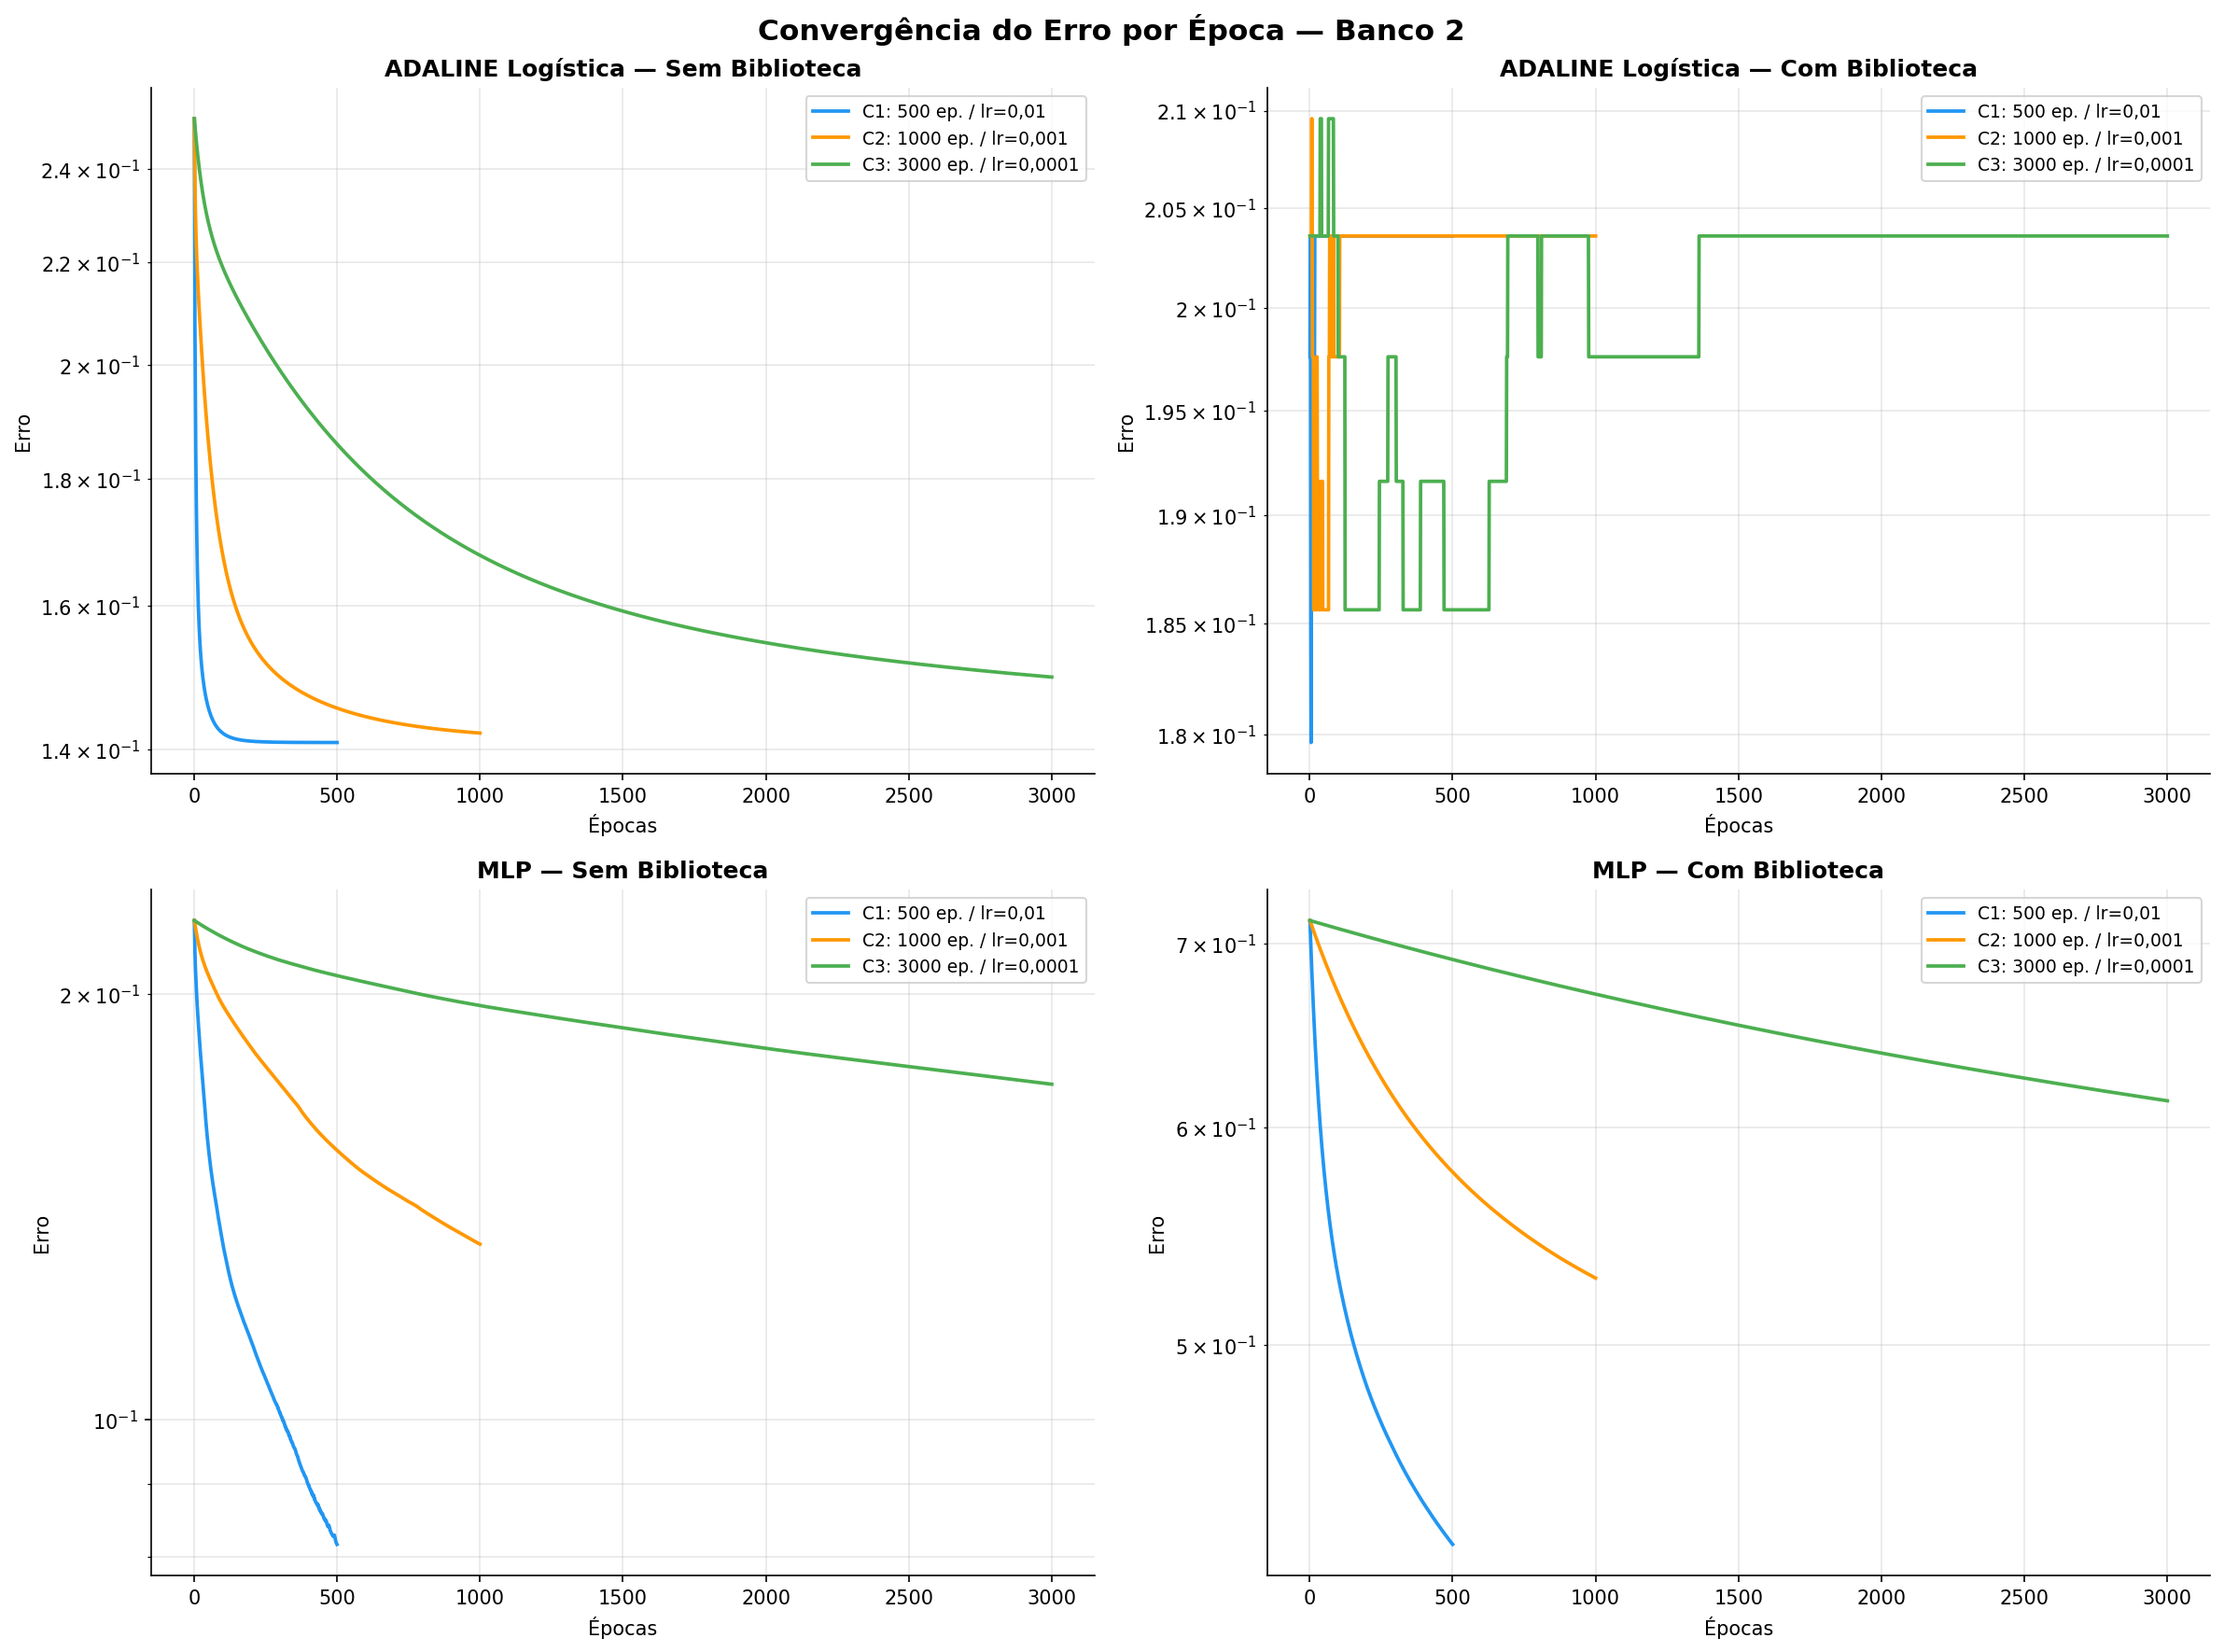
\includegraphics[width=\textwidth]{figuras/resultados/06_convergencia_erro_banco2.png}
\fonte{Elaborado pelo autor.}
\end{figure}

A Figura~\ref{fig:convergencia_banco2} reforça o diagnóstico de \textit{overfitting} nos modelos MLP; os modelos ADALINE convergem de forma suave e estável, coerentemente com seus resultados de acurácia.

Para o MLP NumPy e o MLP Sklearn, o que chama atenção é a velocidade de decrescimento do erro de treino em C1 para ambos: com apenas 500 épocas e taxa $\eta = 0{,}01$, o erro de treinamento cai rapidamente, mais depressa do que nos outros bancos de dados, o que é esperado em conjuntos menores, onde há menos padrões para aprender. Porém, à medida que o número de épocas aumenta (C3), o erro de treino continua decrescendo mesmo quando o desempenho no conjunto de teste piorou, caracterizando o \textit{overfitting}. Esse comportamento é especialmente pronunciado no MLP Sklearn em C3, cujo erro de treinamento é o menor de todos os modelos, mas cuja acurácia de teste é a pior (63,33\%).

\section{Síntese Comparativa entre Modelos e Bancos de Dados}
\label{sec:comparativo}

A visão consolidada dos 24 experimentos é apresentada nas Figuras~\ref{fig:comp_acuracia}, \ref{fig:comp_fn} e \ref{fig:painel_resumo}. A Figura~\ref{fig:comp_acuracia} exibe a acurácia percentual de cada modelo nas três configurações para os dois bancos, permitindo identificar tendências de melhora ou degradação ao longo do treinamento. A Figura~\ref{fig:comp_fn} apresenta o correspondente número de Falsos Negativos, complementando a análise sob o critério clínico prioritário. A Figura~\ref{fig:painel_resumo} resume ambas as métricas exclusivamente para a configuração C3, adotada como referência de comparação final por representar o regime de treinamento mais longo.

\begin{figure}[H]
\centering
\caption{Comparativo de acurácia dos quatro modelos nas três configurações, para os dois bancos de dados.}
\label{fig:comp_acuracia}
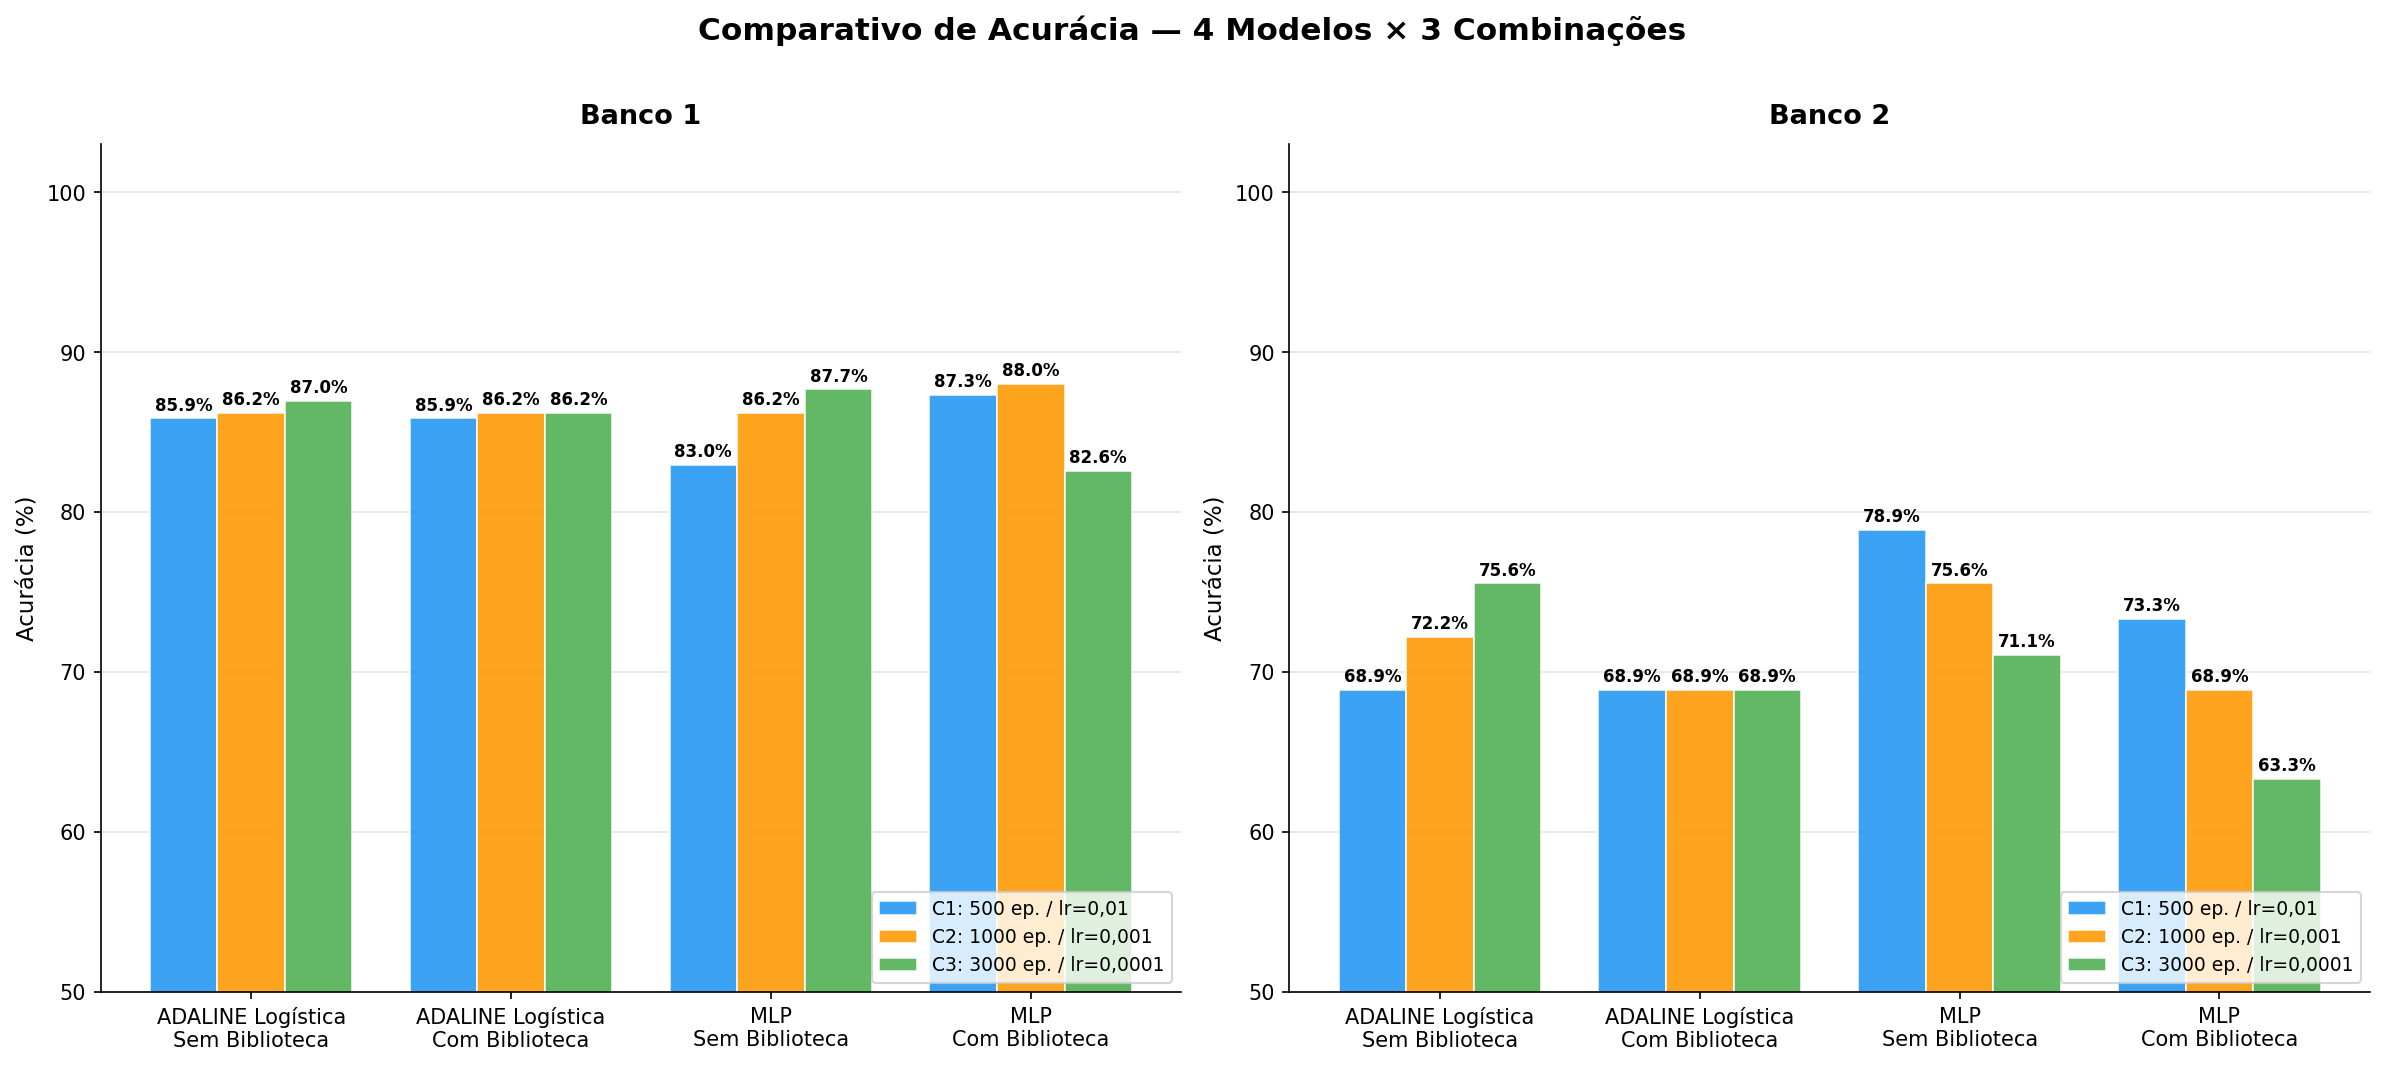
\includegraphics[width=\textwidth]{figuras/resultados/01_comparativo_acuracia.png}
\fonte{Elaborado pelo autor.}
\end{figure}

\begin{figure}[H]
\centering
\caption{Comparativo de Falsos Negativos dos quatro modelos nas três configurações, para os dois bancos de dados.}
\label{fig:comp_fn}
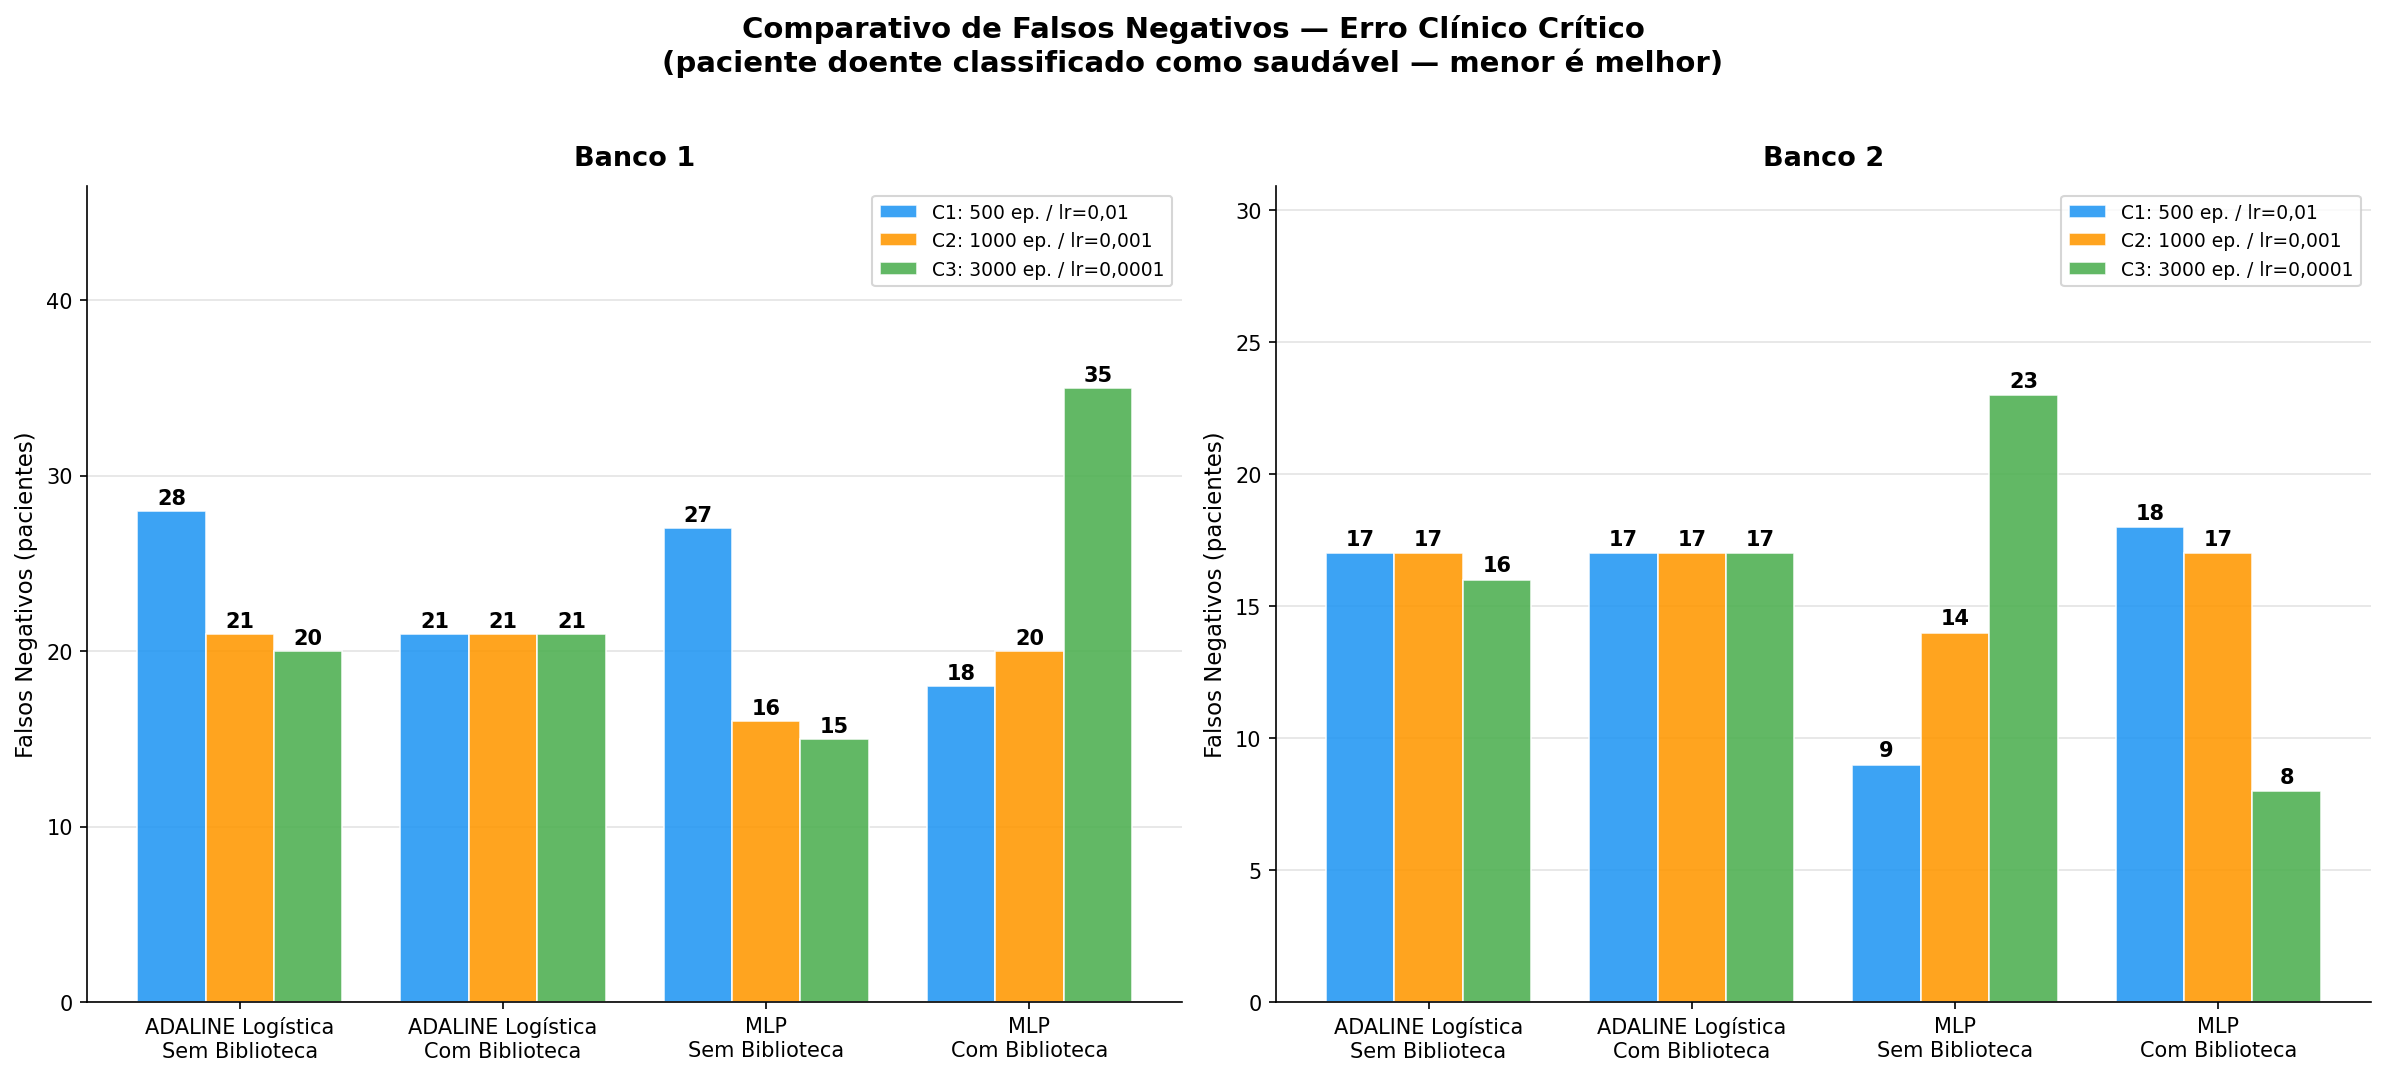
\includegraphics[width=\textwidth]{figuras/resultados/02_comparativo_falsos_negativos.png}
\fonte{Elaborado pelo autor.}
\end{figure}

\begin{figure}[H]
\centering
\caption{Painel resumo comparativo da configuração C3 (3.000 épocas, $\eta$ = 0,0001) para os dois bancos de dados: acurácia (superior) e Falsos Negativos (inferior).}
\label{fig:painel_resumo}
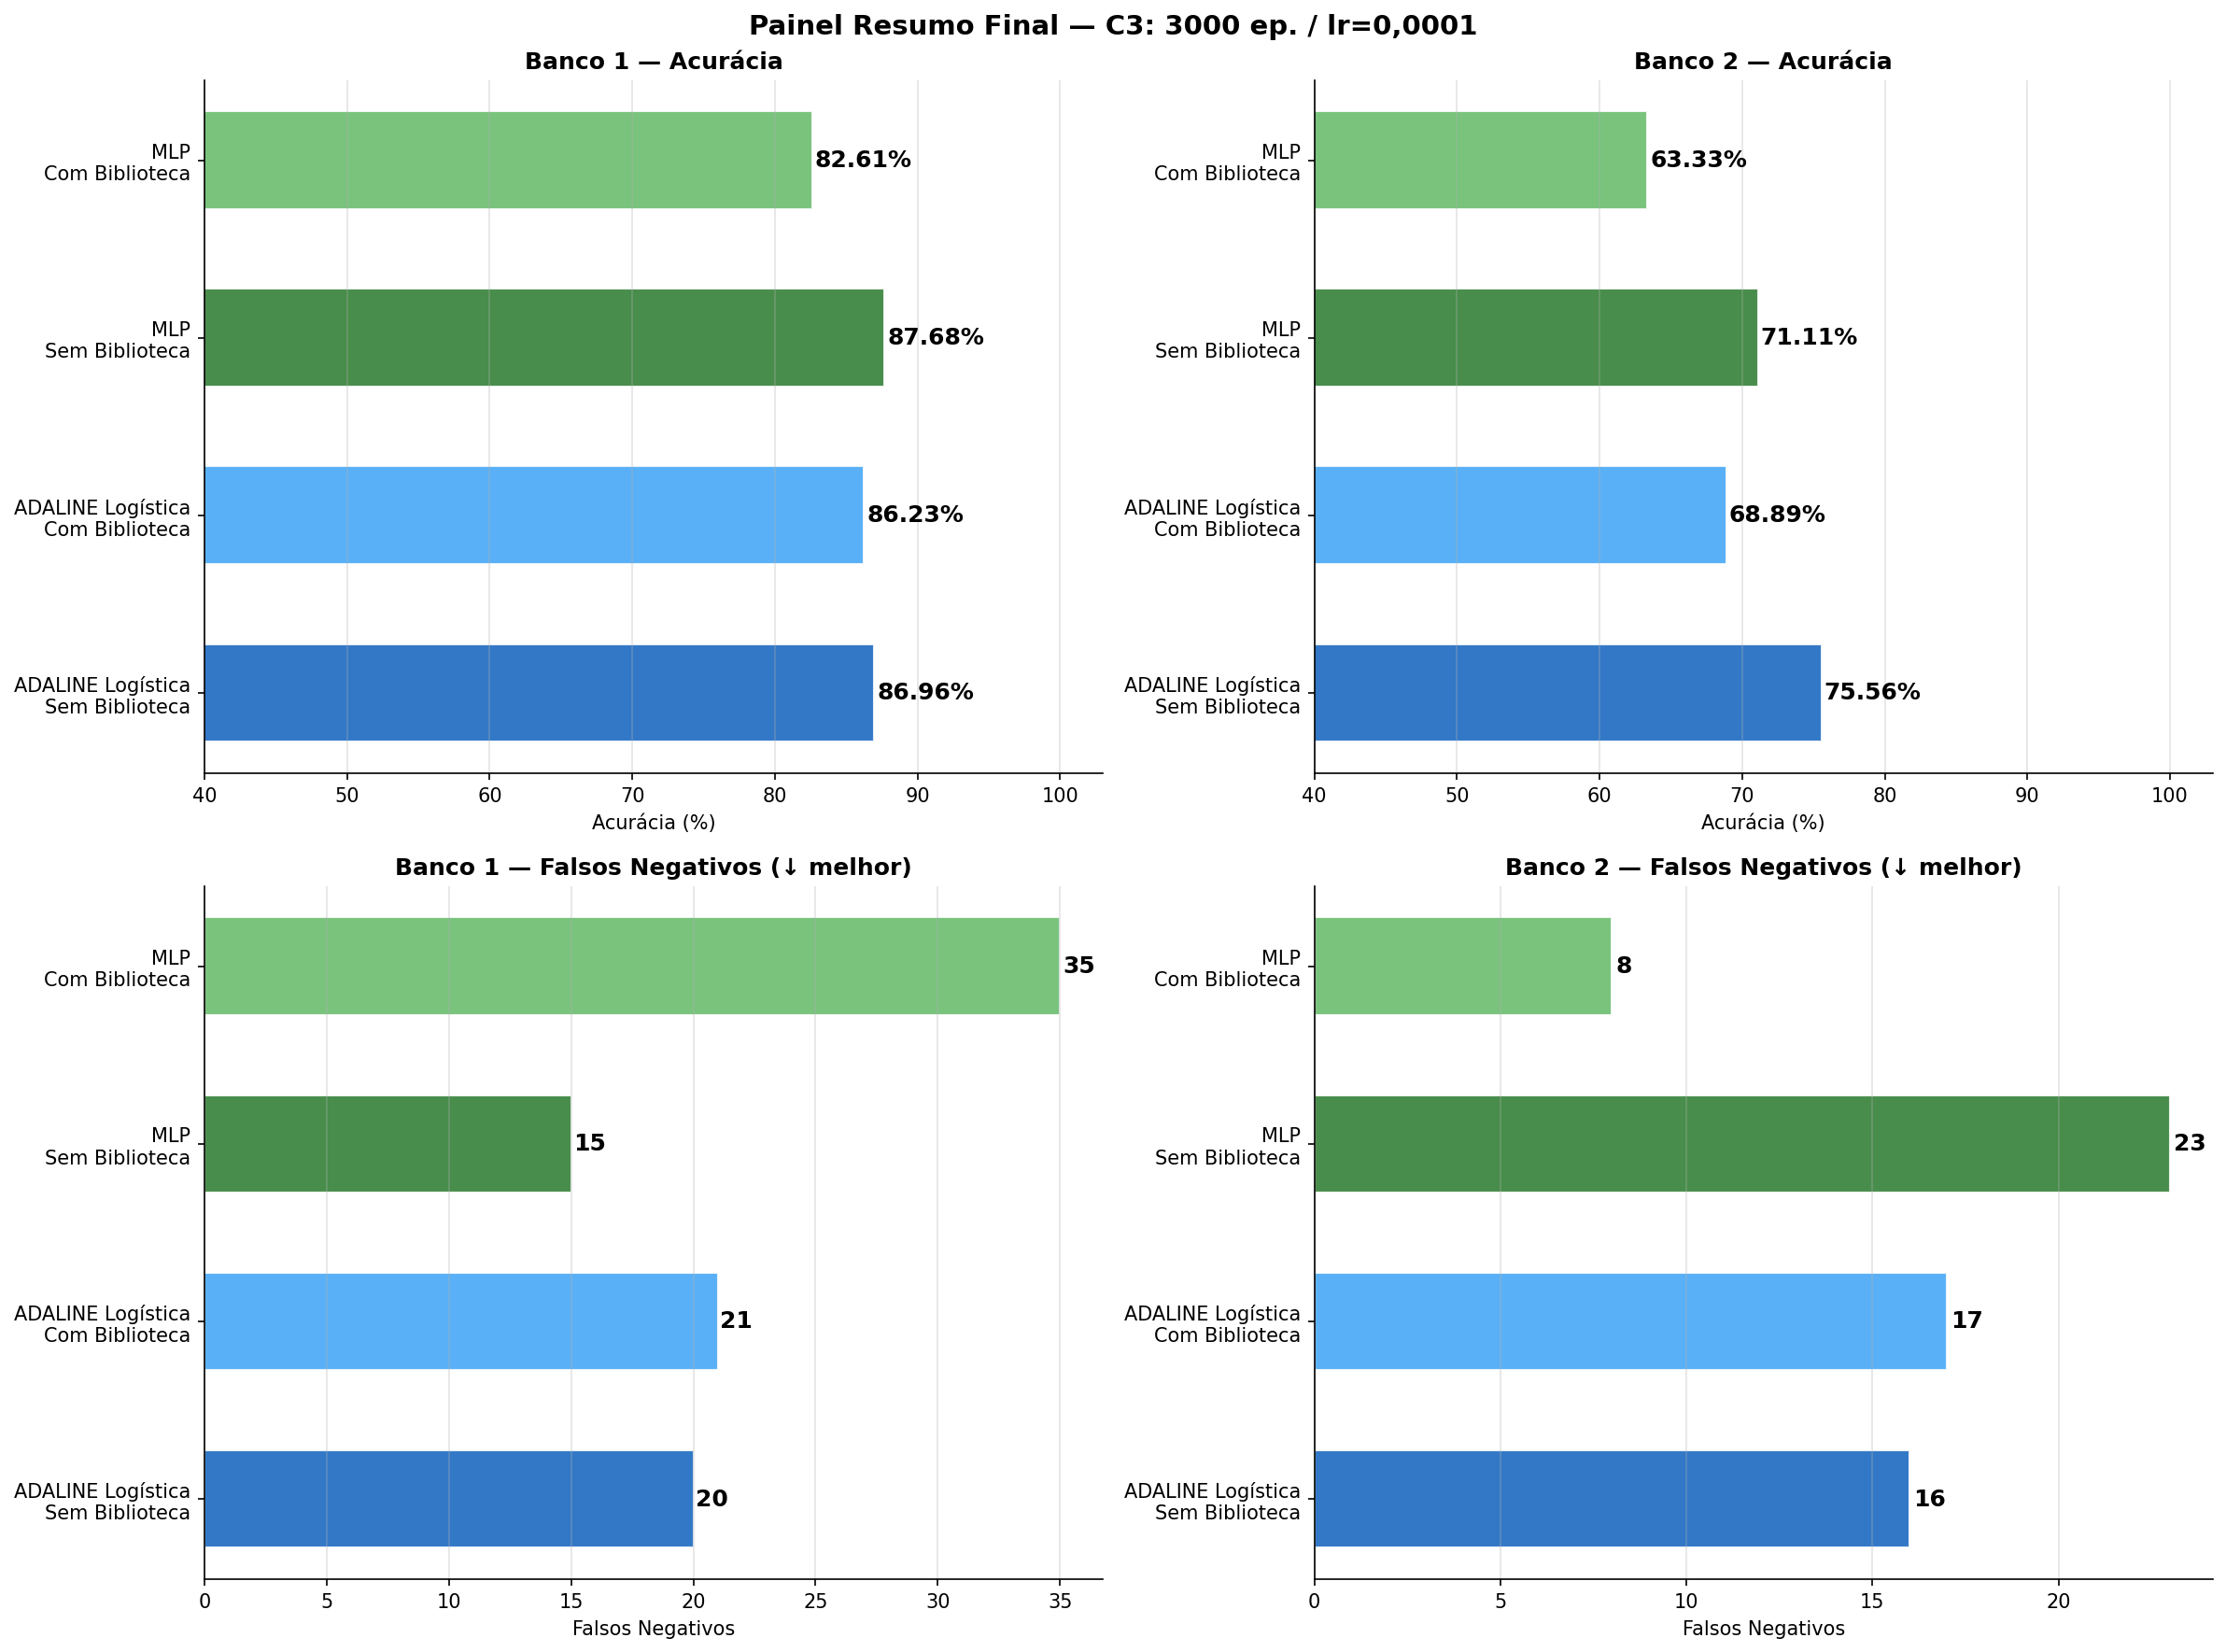
\includegraphics[width=\textwidth]{figuras/resultados/09_painel_resumo_final.png}
\fonte{Elaborado pelo autor.}
\end{figure}

A Tabela~\ref{tab:resumo_geral} sintetiza os melhores resultados por critério e banco de dados.

\begin{table}[H]
\centering
\caption{Síntese dos melhores resultados por critério e banco de dados.}
\label{tab:resumo_geral}
\begin{tabular}{|l|l|c|c|}
\hline
\textbf{Banco} & \textbf{Critério} & \textbf{Melhor modelo / config.} & \textbf{Valor} \\
\hline
Banco 1 & Maior acurácia         & MLP Sklearn C2        & 88,04\% \\
Banco 1 & Menor FN (clínico)     & MLP NumPy C3          & 15 FNs (Sens. 90,20\%) \\
Banco 2 & Maior acurácia         & MLP NumPy C1          & 78,89\% \\
Banco 2 & Menor FN (clínico)     & MLP Sklearn C3        & 8 FNs (Sens. 72,41\%) \\
Banco 2 & Melhor equilíbrio      & MLP NumPy C1          & 78,89\% / 9 FNs \\
\hline
\end{tabular}
\fonte{Elaborado pelo autor.}
\end{table}

\subsection{Considerações Finais sobre os Resultados}
\label{sec:consideracoes_resultados}

\begin{itemize}
    \item No Banco 1, o MLP NumPy em C3 é o modelo recomendado sob o critério clínico de minimização de Falsos Negativos: 87,68\% de acurácia e 15 FNs, com sensibilidade de 90,20\%. O MLP Sklearn em C2 é o melhor em acurácia absoluta (88,04\%), mas com maior FN (20).

    \item No Banco 2, o MLP NumPy em C1 oferece o melhor equilíbrio geral: 78,89\% de acurácia e 9 FNs, com sensibilidade de 68,97\%. Configurações mais longas causam \textit{overfitting} evidente neste modelo.

    \item O ADALINE NumPy mostrou comportamento consistente e previsível nos dois bancos, com melhora gradual e sem degradação em nenhuma configuração. Sua estabilidade o torna adequado em cenários onde a confiabilidade do comportamento é prioridade.

    \item O ADALINE Sklearn apresentou rigidez de comportamento com FNs idênticos em todas as configurações do Banco 2 e acurácia estacionária, limitando sua utilidade em cenários que exigem ajuste fino.

    \item A superioridade esperada do MLP sobre o ADALINE não se materializou de forma consistente, em razão do volume limitado de dados e da instabilidade do SGD com momento em datasets pequenos com muitas épocas, fatores confirmados empiricamente pelo experimento complementar da Seção~\ref{sec:resultados_bruto}, que descartou a binarização como fator determinante.
\end{itemize}

\section{Experimento Complementar: Dados Originais sem Binarização}
\label{sec:resultados_bruto}

Para verificar o efeito da binarização sobre o desempenho relativo dos modelos, os quatro algoritmos foram reaplicados sobre os dados brutos, substituindo a binarização clínica por \textit{one-hot encoding} para as variáveis categóricas do Banco~1 e padronização \textit{z-score} (\texttt{StandardScaler}) para as variáveis numéricas. O Banco~1 resultou em 18 características (contra 35 do experimento binarizado) e o Banco~2 em 12 (contra 14). A divisão treino/validação/teste e as três configurações foram mantidas idênticas ao experimento principal.

\subsection{Resultados no Banco 1 com Dados Brutos}
\label{sec:bruto_banco1}

A Tabela~\ref{tab:bruto_banco1} apresenta a acurácia e o número de Falsos Negativos obtidos pelos quatro modelos nas três configurações, com dados brutos do Banco~1.

\begin{table}[H]
\centering
\caption{Acurácia (\%) e Falsos Negativos (FN), Banco 1, dados brutos. Conjunto de teste: 276 pacientes.}
\label{tab:bruto_banco1}
\resizebox{\textwidth}{!}{%
\begin{tabular}{|l|c|c|c|c|c|c|}
\hline
\multirow{2}{*}{\textbf{Modelo}} & \multicolumn{2}{c|}{\textbf{C1 (500 ep. / $\eta$=0,01)}} & \multicolumn{2}{c|}{\textbf{C2 (1000 ep. / $\eta$=0,001)}} & \multicolumn{2}{c|}{\textbf{C3 (3000 ep. / $\eta$=0,0001)}} \\
\cline{2-7}
 & \textbf{Acurácia} & \textbf{FN} & \textbf{Acurácia} & \textbf{FN} & \textbf{Acurácia} & \textbf{FN} \\
\hline
ADALINE NumPy   & 87,68\% & 16 & 87,68\% & 16 & 87,68\% & 16 \\
ADALINE Sklearn & 88,04\% & 15 & 87,32\% & 16 & 87,68\% & 16 \\
MLP NumPy       & 86,96\% & 16 & 87,32\% & 17 & \textbf{88,77\%} & \textbf{14} \\
MLP Sklearn     & 86,59\% & 14 & 86,59\% & 16 & 81,52\% & 22 \\
\hline
\end{tabular}}
\fonte{Elaborado pelo autor.}
\end{table}

No Banco~1, o ADALINE NumPy convergiu para 87,68\% em todas as configurações (superior ao melhor binarizado, 86,96\%), e o MLP NumPy atingiu 88,77\% / 14~FNs em C3, superando seu melhor resultado binarizado (87,68\% / 15~FNs). O MLP Sklearn manteve a instabilidade em C3 (81,52\%, 22~FNs), replicando o padrão do experimento principal.

\subsection{Resultados no Banco 2 com Dados Brutos}
\label{sec:bruto_banco2}

A Tabela~\ref{tab:bruto_banco2} apresenta os resultados do Banco~2 com dados brutos.

\begin{table}[H]
\centering
\caption{Acurácia (\%) e Falsos Negativos (FN), Banco 2, dados brutos. Conjunto de teste: 90 pacientes (29 óbitos / 61 sobreviventes).}
\label{tab:bruto_banco2}
\resizebox{\textwidth}{!}{%
\begin{tabular}{|l|c|c|c|c|c|c|}
\hline
\multirow{2}{*}{\textbf{Modelo}} & \multicolumn{2}{c|}{\textbf{C1 (500 ep. / $\eta$=0,01)}} & \multicolumn{2}{c|}{\textbf{C2 (1000 ep. / $\eta$=0,001)}} & \multicolumn{2}{c|}{\textbf{C3 (3000 ep. / $\eta$=0,0001)}} \\
\cline{2-7}
 & \textbf{Acurácia} & \textbf{FN} & \textbf{Acurácia} & \textbf{FN} & \textbf{Acurácia} & \textbf{FN} \\
\hline
ADALINE NumPy   & \textbf{82,22\%} & \textbf{11} & \textbf{82,22\%} & \textbf{11} & \textbf{82,22\%} & \textbf{11} \\
ADALINE Sklearn & 83,33\% & 11 & 83,33\% & 11 & 82,22\% & 11 \\
MLP NumPy       & 80,00\% & 12 & 81,11\% & 12 & 78,89\% & 14 \\
MLP Sklearn     & 81,11\% & 11 & 66,67\% & 15 & 45,56\% & 10 \\
\hline
\end{tabular}}
\fonte{Elaborado pelo autor.}
\end{table}

No Banco~2, os dados brutos trouxeram ganhos expressivos para os ADALINEs: o ADALINE NumPy atingiu 82,22\% / 11~FNs em todas as configurações e o ADALINE Sklearn 83,33\% em C1 e C2, contra a faixa de 68,89\%--75,56\% do experimento binarizado. O ganho de até 14 pontos percentuais demonstra que os biomarcadores contínuos do Banco~2 carregam informação prognóstica que a discretização por limiar clínico não captura. Os MLPs não se beneficiaram dos dados brutos: o MLP NumPy degradou-se de 80,00\% (C1) para 78,89\% (C3), e o MLP Sklearn colapsou para 45,56\% em C3, o pior resultado de todos os 24 experimentos realizados.

\subsection{Comparação: Binarizado versus Bruto}
\label{sec:comparativo_binarizado_bruto}

A Figura~\ref{fig:comparativo_binarizado_vs_bruto} apresenta a comparação direta dos resultados binarizados e brutos na configuração C3 para os dois bancos, em termos de acurácia e Falsos Negativos. As Figuras~\ref{fig:acuracia_bruto} e \ref{fig:fn_bruto} complementam essa análise exibindo, respectivamente, a acurácia e os Falsos Negativos nas três configurações de treinamento com dados brutos.

\begin{figure}[H]
\centering
\caption[Comparativo binarizado vs.\ bruto, configuração C3.]{Comparativo entre o experimento principal (dados binarizados) e o experimento complementar (dados brutos + StandardScaler) na configuração C3, para os dois bancos de dados. Painel superior: acurácia (\%); painel inferior: Falsos Negativos.}
\label{fig:comparativo_binarizado_vs_bruto}
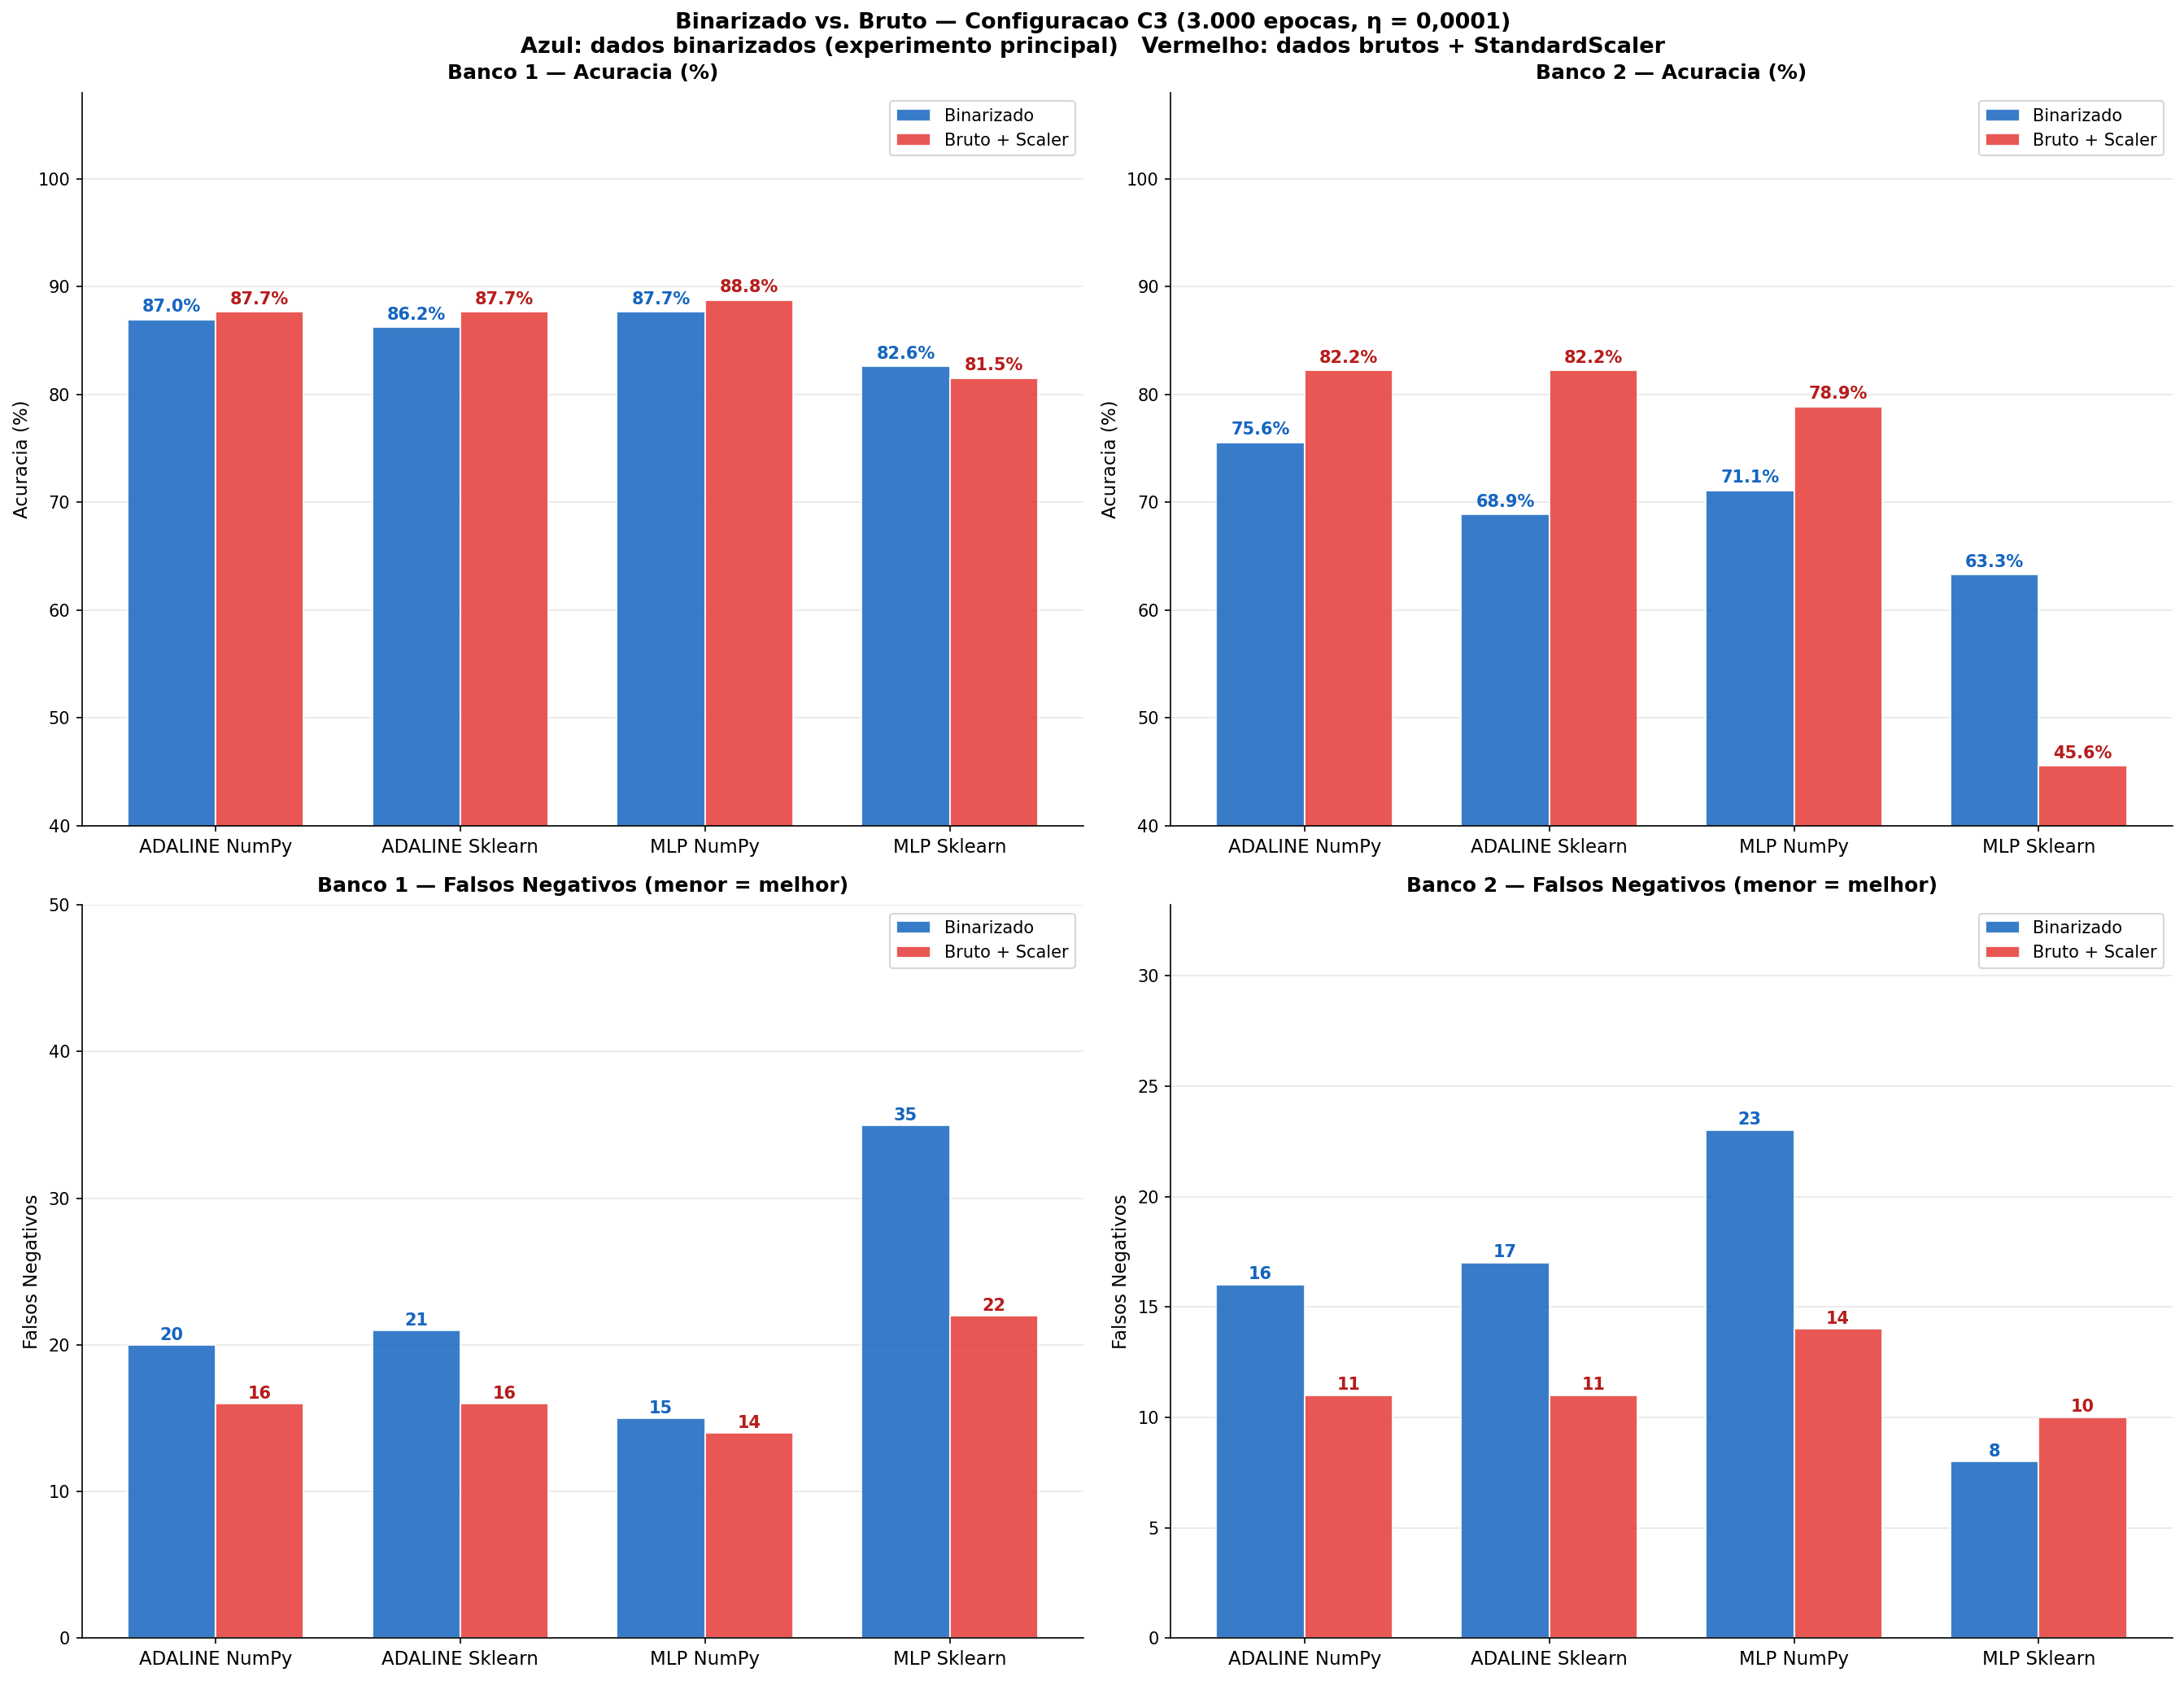
\includegraphics[width=\textwidth]{figuras/resultados/10_comparativo_binarizado_vs_bruto.png}
\fonte{Elaborado pelo autor.}
\end{figure}

\begin{figure}[H]
\centering
\caption{Acurácia dos quatro modelos nas três configurações de treinamento, com dados brutos e StandardScaler.}
\label{fig:acuracia_bruto}
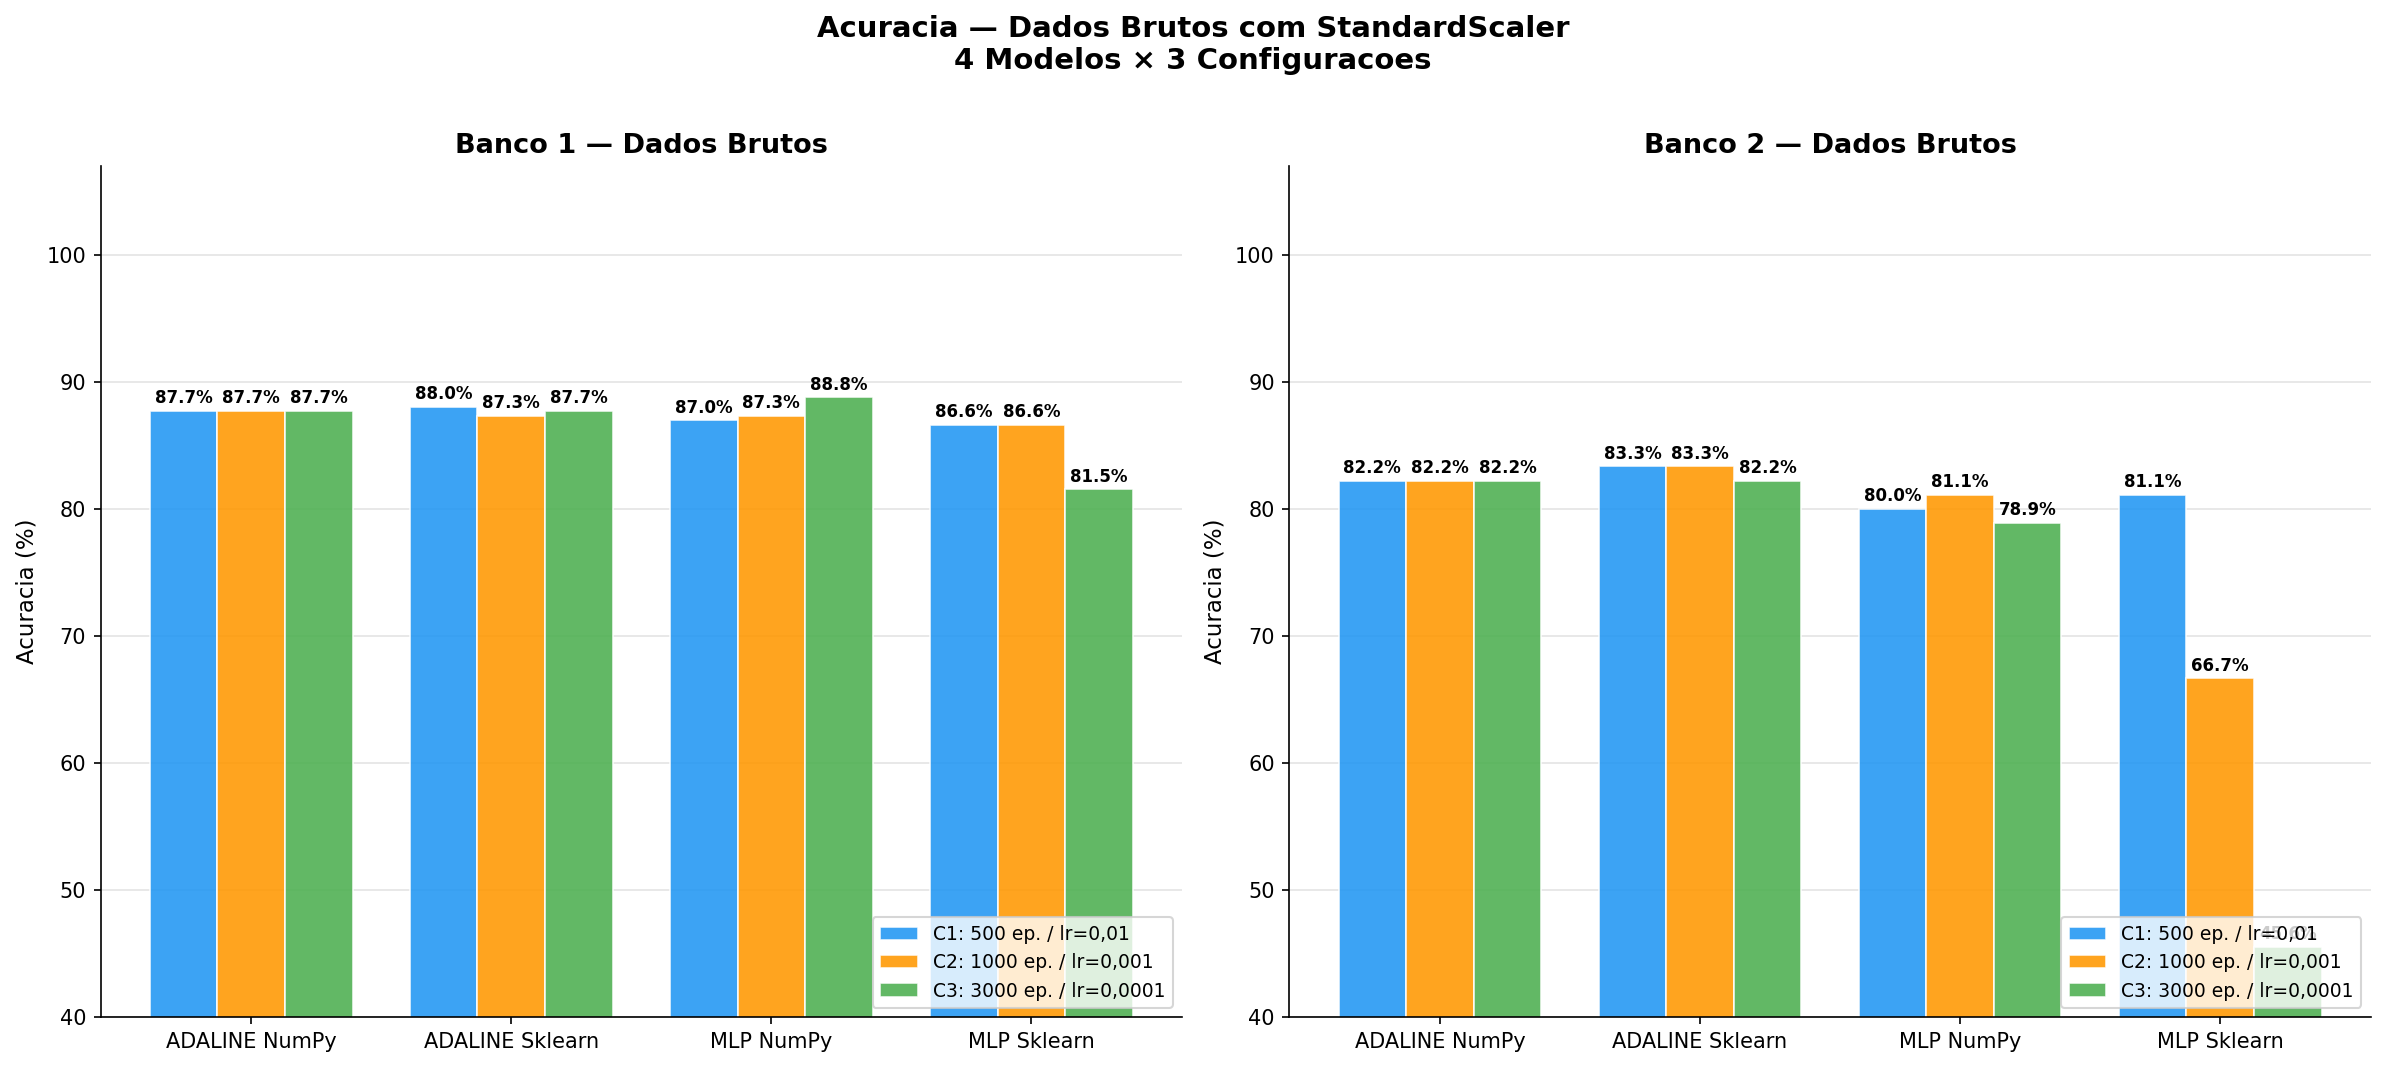
\includegraphics[width=\textwidth]{figuras/resultados/11_acuracia_bruto.png}
\fonte{Elaborado pelo autor.}
\end{figure}

\begin{figure}[H]
\centering
\caption{Falsos Negativos dos quatro modelos nas três configurações de treinamento, com dados brutos e StandardScaler.}
\label{fig:fn_bruto}
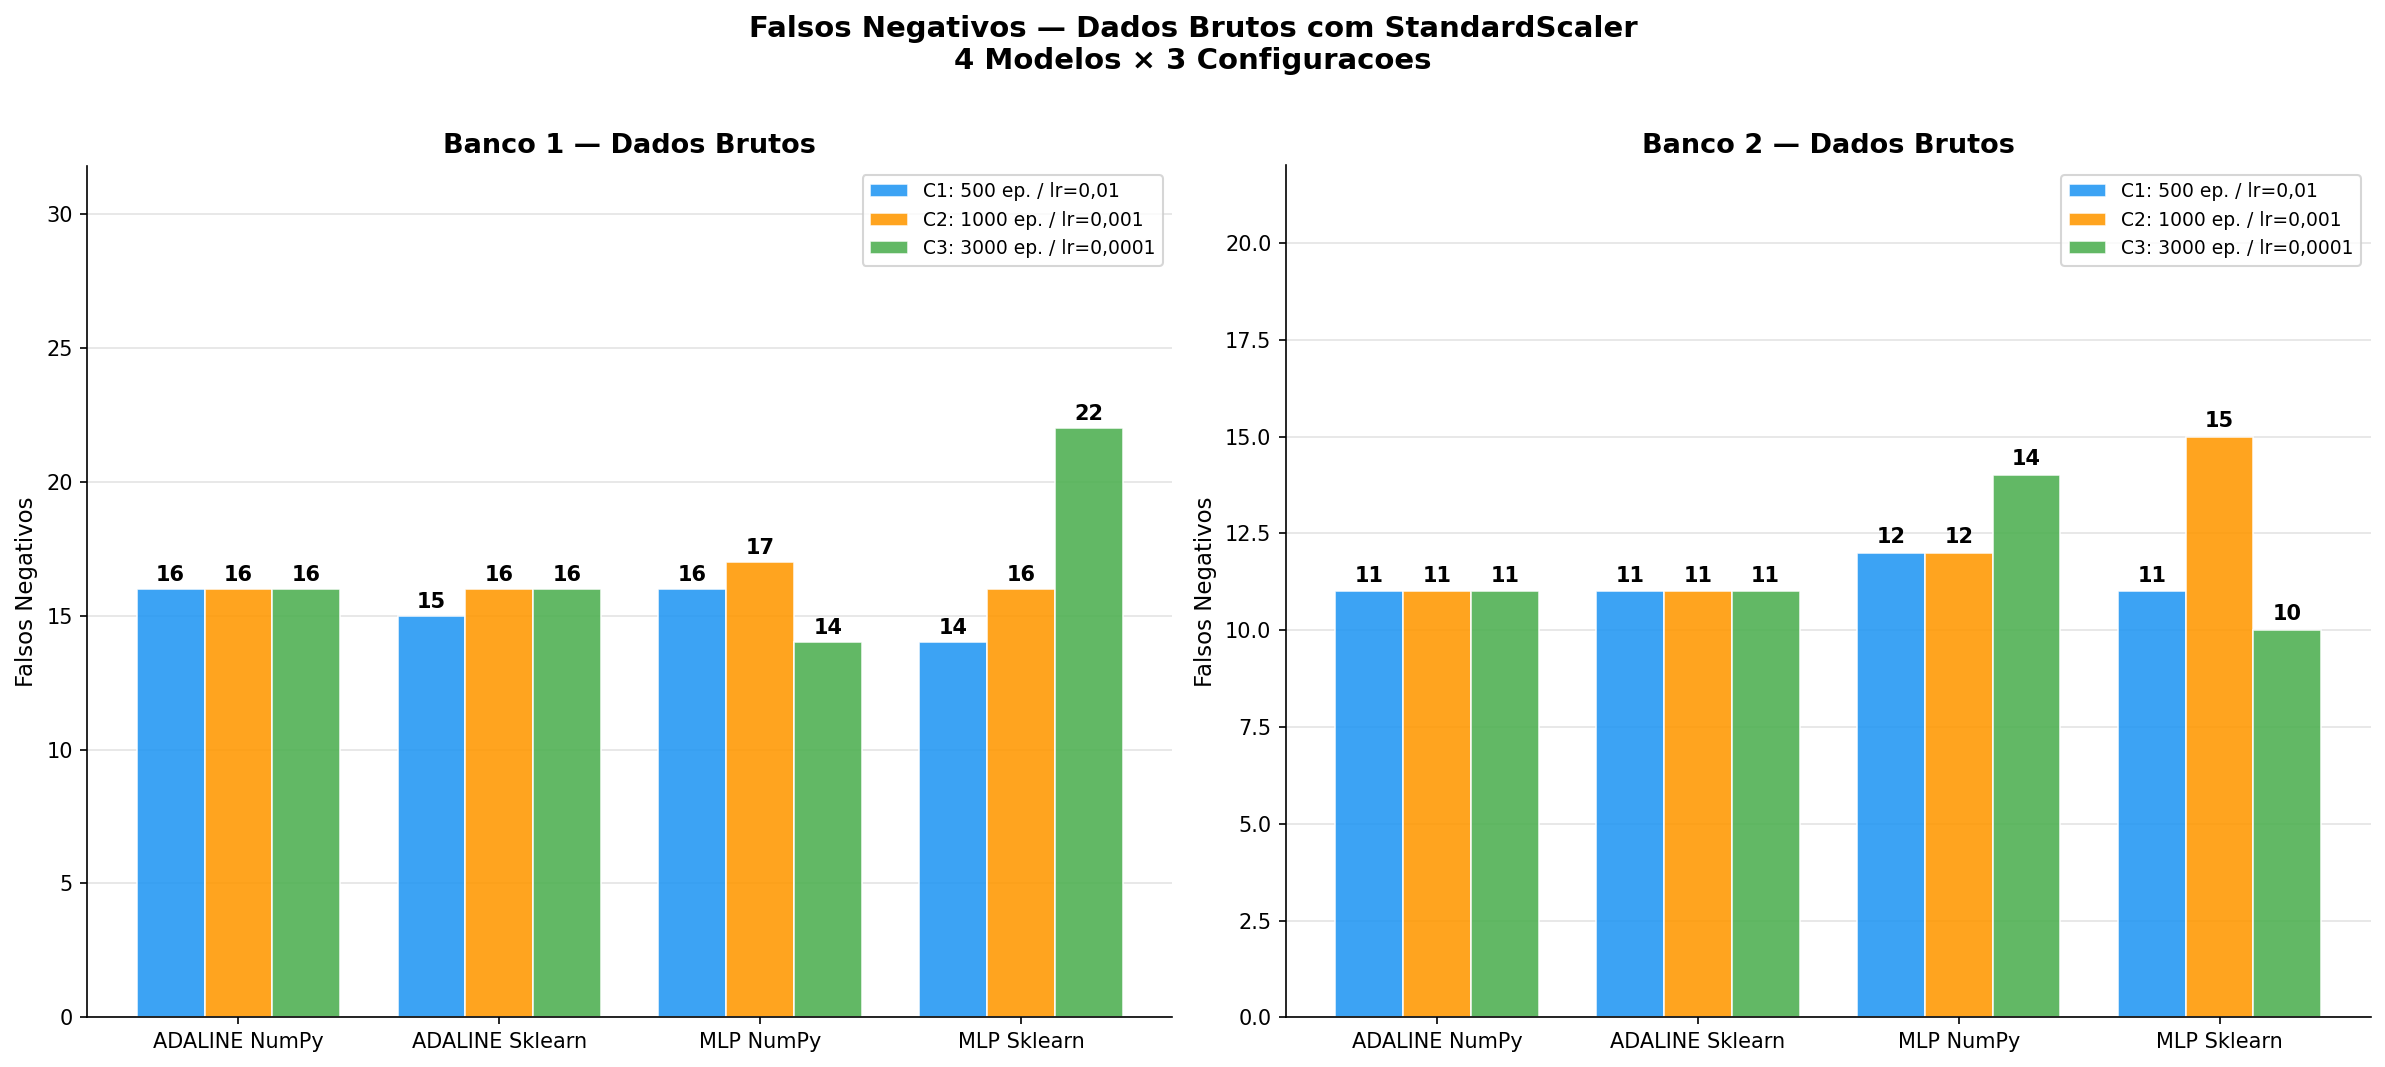
\includegraphics[width=\textwidth]{figuras/resultados/12_fn_bruto.png}
\fonte{Elaborado pelo autor.}
\end{figure}

A conclusão deste experimento é que a binarização não foi a principal responsável pela competitividade do ADALINE: mesmo com dados contínuos, os ADALINEs se mostraram mais estáveis e, no Banco~2, mais acurados do que os MLPs. O fator determinante é o volume de dados disponível para o treinamento, que favorece sistematicamente o modelo mais simples. A persistência da vantagem do ADALINE com representação contínua é consistente com a hipótese de que a fronteira de decisão nesses dados é predominantemente linear, embora o volume reduzido de treinamento impeça confirmar categoricamente essa interpretação. Essa questão é retomada na Seção~\ref{sec:discussao_mlp}.
